\documentclass[letterpaper]{article} % DO NOT CHANGE THIS
\usepackage[submission]{aaai2027}  % DO NOT CHANGE THIS
\usepackage[hyphens]{url}  % DO NOT CHANGE THIS
\usepackage{graphicx} % DO NOT CHANGE THIS
\urlstyle{rm} % DO NOT CHANGE THIS
\def\UrlFont{\rm}  % DO NOT CHANGE THIS
\usepackage{natbib}  % DO NOT CHANGE THIS AND DO NOT ADD ANY OPTIONS TO IT
\usepackage{caption} % DO NOT CHANGE THIS AND DO NOT ADD ANY OPTIONS TO IT
\frenchspacing  % DO NOT CHANGE THIS
\usepackage{booktabs}
\usepackage{array}
\usepackage{amsmath,amssymb,amsthm}
\usepackage{pgfplots}
\pgfplotsset{compat=1.18}
\usepgfplotslibrary{groupplots}
\usetikzlibrary{arrows.meta,positioning,calc}

\pdfinfo{
/TemplateVersion (2027.1)
}

\setcounter{secnumdepth}{2}

\definecolor{cD}{HTML}{0072B2}
\definecolor{cE}{HTML}{D55E00}
\definecolor{cS}{HTML}{009E73}
\definecolor{cP}{HTML}{56B4E9}
\definecolor{cF}{HTML}{CC79A7}
\definecolor{cI}{HTML}{E69F00}
\definecolor{cH}{HTML}{D55E00}

\newtheorem{proposition}{Proposition}
\newtheorem{corollary}{Corollary}
\newtheorem{lemma}{Lemma}
\theoremstyle{definition}
\newtheorem{definition}{Definition}
\newtheorem{remark}{Remark}

\newcommand{\hull}{\operatorname{hull}}
\newcommand{\core}{\operatorname{core}}
\newcommand{\dD}{\mathsf{D}}
\newcommand{\dE}{\mathsf{E}}
\newcommand{\dS}{\mathsf{S}}
\newcommand{\dP}{\mathsf{P}}
\newcommand{\dF}{\mathsf{F}}
\newcommand{\dI}{\mathsf{I}}
\newcommand{\cC}{\mathcal{C}}
\newcommand{\cQ}{\mathcal{Q}}
\newcommand{\cS}{\mathcal{S}}
\newcommand{\Valarm}{V_{\mathrm{alarm}}}

\title{Selecting the Selectors: Recursive Selection and the Evolution of Control over AI Evaluation}
\author{Anonymous Submission}
\affiliations{}

\begin{document}

\maketitle

\begin{abstract}
AI systems are increasingly selected by benchmarks, evaluators, reward models and standards that the most successful developers help to build, fund or supply. We ask when selection itself favors practices that acquire control over later selection. In a model where carriers of a practice vary heritably in their capacity to convert success into rule support, selection favors greater capacity exactly when the appropriable, persistence-weighted return exceeds its marginal cost; when rule support is a shared good, correction is fast or returns arrive late, it does not. The return is a quadratic form in the carrier's success across domains whose kernel is the cross-domain conversion that also decides whether capture is stable, so cross-domain presence, characteristic of general-purpose AI, amplifies it. Selection on capacity can therefore carry a field across its capture threshold with no change in costs or in incidental coupling. For coupled domains we give decentralized and exact certificates against capture, identify which reforms unravel a captured configuration and which are re-absorbed, and show that evaluators drawn from the evaluated lineage delay detection of harm by an amount that diverges at a computable masking level. We derive tests that separate these mechanisms, and governance principles that include lowering the appropriability of rule-making.
\end{abstract}

\section{Introduction}

Frontier AI systems are increasingly selected by processes that their most successful developers help to shape. Benchmarks are assembled from deployed systems and run on developer tooling. Independent evaluators depend on access terms set by the firms they evaluate \citep{longpre2024}, and public leaderboards can favor providers able to test many private variants \citep{singh2025}. Language-model judges and reward models now decide much of what counts as a good output; they favor outputs related to their own lineage \citep{panickssery2024,li2026preference,awuni2026} and share errors across providers \citep{kim2025,goel2025}. The processes that decide which systems, practices and organizations expand are partly products of earlier winners.

Such feedback is usually studied as entrenchment: success shapes the conditions of future success \citep{arthur1989,pierson2000,acemoglu2008,hardt2022}. This paper asks a prior question: \emph{when does selection itself favor practices that acquire control over later selection?} Rule support is not only a by-product of success; it is cultivated. Organizations differ in how much they invest in drafting standards, building evaluation infrastructure, authoring benchmarks and securing dependencies, and these investments are costly. If they pay, the capacity to reshape selection is itself selected, and capture becomes something selection produces rather than something that occasionally happens. If they do not, because the benefits leak to competitors, correction is fast or returns arrive too late, rule support stays incidental.

Our central result (Section~\ref{sec:capacity}) says which case obtains. When carriers of a practice vary heritably in conversion capacity, selection favors greater capacity exactly when the appropriable, persistence-weighted return to it exceeds its marginal cost. The return is a quadratic form in the carrier's success across domains, and its kernel is the cross-domain conversion that also decides whether capture of a domain is stable. Capture and selection for capacity therefore reinforce each other, and selection on capacity alone can carry a field of coupled domains across its capture threshold. The remaining results concern such fields: when local audits can certify them, which reforms unravel a captured configuration, and how capture of evaluation delays or silences the detection of harm (Sections~\ref{sec:field}--\ref{sec:selectors}).

General-purpose AI plausibly moves each quantity in these conditions (Section~\ref{sec:ai}). Its developers are present in many domains at once, which amplifies the return to capacity; capable assistants lower the cost of drafting, lobbying and writing evaluations; and AI judges put the evaluated lineage in the selector's seat. Aligning each system to its operator does not bound any of this: an assistant that serves its principal faithfully lowers exactly the costs that decide whether control capacity is selected.

The paper makes four contributions: (1) a value-neutral definition of regimes in which success maintains its own selection conditions, with pathology as separate conditions (Section~\ref{sec:framework}); (2) a conditional theorem on selection for conversion capacity, with counterexamples, a scope result, an assistance result and a ratchet linking capacity to capture thresholds (Section~\ref{sec:capacity}); (3) for coupled domains, certificates, a seed-conditioned cascade, reform and keystone results, and a detection-delay law (Sections~\ref{sec:field}--\ref{sec:selectors}); (4) a mapping to AI oversight, discriminating tests and governance principles (Sections~\ref{sec:ai}--\ref{sec:design}).

\paragraph{Statement of Contributions.} The novelty lies in the conditional result on selection for conversion capacity and its coupling to cross-domain capture thresholds (Section~\ref{sec:capacity}), in the certificates, keystone sets and detection-delay law for coupled domains (Sections~\ref{sec:field}--\ref{sec:selectors}), and in their application to AI evaluation and governance. The tools are standard: replicator dynamics, the Price equation and comparison theorems for monotone systems; the field results are continuous-time analogues of threshold-cascade and $k$-core results, which we cite. Conceptual antecedents of Section~\ref{sec:framework} appeared in informal, non-peer-reviewed essays; all formal content is new and unpublished.

\section{Related Work}\label{sec:related}

\paragraph{Structural and multi-agent risk.} AI can cause harm by changing incentives rather than through accident or misuse \citep{zwetsloot2019}; optimizing measurable proxies can erode human influence gradually \citep{christiano2019,kulveit2025,kasirzadeh2025}; aligning each system to its principal leaves the game between principals unaligned \citep{critch2020,critch2023,dafoe2020}; processes can persist whichever agents carry them \citep{critch2021}; and selection pressures among AI systems can favor undesirable traits \citep{hendrycks2023,hammond2025}. We inherit the thesis that per-system alignment does not bound field-level outcomes and contribute a mechanism with conditions.

\paragraph{Capture.} Industry influence over regulators \citep{stigler1971,dalbo2006,carpenter2013} can work without intent, through shared worldviews and status \citep{kwak2014}, and can reach how problems are framed \citep{hanson2003}; de facto power can offset changes in de jure institutions \citep{acemoglu2008}; firm expertise converts into standard-setting power \citep{buthe2011}; and agenda-setting, academic capture and information management operate in AI policy \citep{wei2024,abdalla2021,whittaker2021,ahmed2023}.

\paragraph{Selection on the rules of selection.} Selection retains the selectors that later filter variation \citep{campbell1974}. Rules that govern future rule-making have been modelled as self-stable constitutions and dynamically stable coalitions \citep{barbera2004,acemoglu2012}, behaviors and institutions co-evolve \citep{bowles2003}, social learning rules evolve \citep{kendal2009}, and institutions can self-organize in evolutionary dynamical-systems games \citep{itao2025}. \citet{kluver2002} used ``meta-attractor'' for the stable state of the rules that generate a system's attractors. Niche construction and eco-evolutionary games with environmental feedback produce coexistence, cycles and alternative stable states \citep{laland1999,odlingsmee2003,weitz2016,tilman2020,ito2024}, and the specificity of niche benefits decides whether niche-constructing traits are selected in tumours \citep{gerlee2015}, the closest precedent for our appropriability condition. Performative prediction and performative power capture how deployed models shape the data that evaluate them \citep{perdomo2020,hardt2022,krueger2020}; measures used for allocation degrade \citep{campbell1979,manheim2018,smaldino2016}.

\paragraph{Cascades.} Threshold cascades, cohesive sets and $k$-cores \citep{granovetter1978,watts2002,morris2000,kempe2003,seidman1983}, anchored and collapsed $k$-cores \citep{bhawalkar2015,zhang2017collapsed}, coupled tipping \citep{brummitt2015} and monotone systems \citep{hirsch1985,smith1995} supply our field-level tools.

\paragraph{AI evaluation and oversight.} Audits face limited access, funding and independence \citep{raji2022,costanzachock2022,birhane2024}. Oversight proposals place AI in the evaluator's seat \citep{irving2018,christiano2018,leike2018,bai2022,burns2024,greenblatt2024}; we connect them to evaluator provenance in Section~\ref{sec:ai}.

\section{Practices, Selectors and Meta-Attractors}\label{sec:framework}

\paragraph{Three levels.} We separate the \emph{outcomes} of selection (which practices expand), the \emph{selection environment} (the rules, evaluations, entry conditions and resources on which outcomes depend), and the \emph{capacity to reshape} that environment. A practice is a reproducible way of succeeding, such as releasing systems before independent evaluation concludes. It is carried by organizations, people and models, and can persist when its carriers change. Our model of the first two levels makes the environment endogenous, as much prior work does; the new step (Section~\ref{sec:capacity}) is heritable variation at the third.

\paragraph{From being selected to selecting the selectors.} Consider a research community that allocates funding and positions by publication counts, because reliable knowledge is hard to evaluate directly. Practices that produce more publications receive more funding, attract more students and are more widely copied \citep{smaldino2016}. Now add one step: their practitioners come to occupy the positions that decide recruitment, training and evaluation. The practice is then no longer only selected by a rule; it helps reproduce the rule that selects it. No manipulation is needed. Ordinary decisions about whom to hire, what to build, what to teach and which dependencies to accept suffice, and what persists can be a way of succeeding rather than any carrier, so replacing the occupants of powerful positions may leave the trajectory unchanged. Two kinds of closure can follow. \emph{Practical closure} makes alternatives hard to sustain. \emph{Epistemic closure} makes their merits, or the practice's harms, hard to represent in ways that affect decisions: a system can retain abundant information while losing the ability to let it change course. When a practice's success shapes the processes that select it, above all those that observe harm and trigger correction, we say that it selects its selectors.

\begin{figure}[t]
\centering
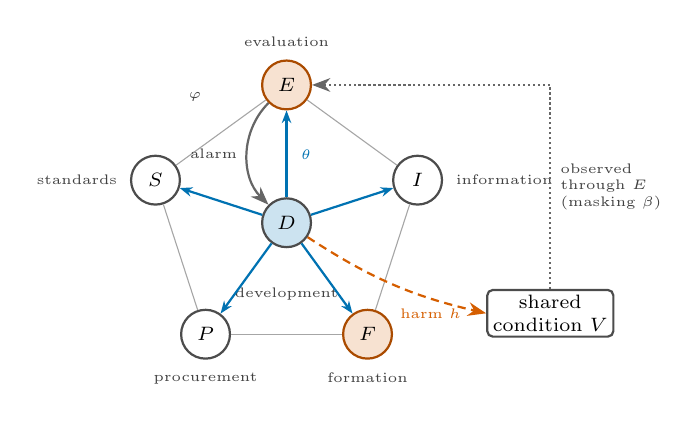
\begin{tikzpicture}[
  dom/.style={circle, draw=black!70, thick, minimum size=0.62cm, inner sep=0pt, font=\scriptsize},
  sel/.style={dom, fill=cE!18, draw=cE!80!black},
  lab/.style={font=\tiny, text=black!75},
  conv/.style={-{Stealth[length=1.6mm]}, thick, cD},
  ring/.style={black!35, thin},
  >=Stealth]
  \def\rr{1.75}
  \node[dom, fill=cD!20] (D) at (0,0) {$D$};
  \node[sel] (E) at (90:\rr) {$E$};
  \node[dom] (I) at (18:\rr) {$I$};
  \node[sel] (F) at (306:\rr) {$F$};
  \node[dom] (P) at (234:\rr) {$P$};
  \node[dom] (S) at (162:\rr) {$S$};
  \node[lab, above=0.4mm of E] {evaluation};
  \node[lab, right=0.4mm of I] {information};
  \node[lab, below=0.4mm of F] {formation};
  \node[lab, below=0.4mm of P] {procurement};
  \node[lab, left=0.4mm of S] {standards};
  \node[lab] at (0,-0.9) {development};
  \foreach \a/\b in {E/I, I/F, F/P, P/S, S/E} {\draw[ring] (\a) -- (\b);}
  \node[lab] at (126:1.98) {$\varphi$};
  \foreach \n in {E, I, F, P, S} {\draw[conv] (D) -- (\n);}
  \node[lab, text=cD] at (74:0.9) {$\theta$};
  \draw[->, black!60, thick] (E.south west) to[out=225, in=135] node[lab, left, pos=0.5] {alarm} (D.north west);
  \node[draw=black!70, thick, rounded corners=2pt, font=\scriptsize, align=center, inner sep=2pt] (V) at (3.35,-1.15) {shared\\condition $V$};
  \draw[->, cH, thick, densely dashed] (D) to[bend right=10] node[lab, text=cH, below, pos=0.72] {harm $h$} (V.west);
  \draw[->, black!60, densely dotted, thick] (V.north) |- node[lab, right, pos=0.25, align=left] {observed\\through $E$\\(masking $\beta$)} (E.east);
\end{tikzpicture}

\caption{The model. Success in development converts into rule support in the other domains ($\theta$), which also convert among themselves ($\varphi$). Carriers with conversion capacity $q$ add cultivated conversion, and the appropriable share $\chi$ of the return, which grows with their success across domains, decides whether capacity is selected (Section~\ref{sec:capacity}). The practice depletes a shared condition $V$ that selection does not see; correction depends on reports through evaluation, which capture masks ($\beta$).}
\label{fig:schematic}
\end{figure}

\paragraph{Model.} There are $n$ selection domains, $N=\{1,\dots,n\}$; for AI, think of development, evaluation, standards, procurement, formation (education, professional training, curated training data) and information, labelled $\dD,\dE,\dS,\dP,\dF,\dI$. In domain $i$ a share $x_i\in[0,1]$ of consequential decisions follows the practice, and \emph{rule support} $r_i\ge0$ measures how far the domain's selection environment favors it: benchmarks built from deployed systems, procurement defaults keyed to incumbent interfaces, evaluation criteria and curricula organized around the practice. The dynamics are
\begin{align}
\dot x_i&=\kappa_i x_i(1-x_i)(a_ir_i-c_i)+\mu(1-2x_i),\label{eq:x}\\
\dot r_i&=\varepsilon_i\Big(\textstyle\sum_{j}b_{ij}x_j-d_ir_i\Big),\label{eq:r}
\end{align}
with positive rates and $b_{ij}\ge0$. Under the \emph{baseline rules} $r=0$ the practice carries a relative cost $c_i$, which rule support offsets at rate $a_i$. The conversion matrix $B=(b_{ij})$ records how success in domain $j$ becomes rule support in domain $i$ through funding, personnel, authorship of standards and benchmarks, data and infrastructure dependence, or access terms; support decays or is corrected at rate $d_i$. Two-way entry at rate $\mu\ge0$ keeps a trickle of the practice and of its alternative in every domain. We state exact results for $\mu=0$; at hyperbolic equilibria they persist with $O(\mu)$ shifts for small $\mu>0$. The payoff difference does not depend on $x_i$, so Eq.~(\ref{eq:x}) is a switch driven by rule support, not a game among adopters. Shares and stocks belong to practices, not to actors.

The \emph{normalized conversion} $R_{ij}=a_ib_{ij}/(c_id_i)$ is the rule support that full adoption in $j$ would generate in $i$, relative to the cost it must offset. For a set $\cC$ of domains, the \emph{inbound conversion} $s_i(\cC)=\sum_{j\in\cC}R_{ij}$ includes $R_{ii}$ when $i\in\cC$. For $n=1$ there is a single threshold $R=ab/(cd)$: if $R<1$ the practice dies out from any state with $x<1$; if $R>1$, absence and full capture are both stable, separated by a curve through $(1/R,c/a)$, so present share and inherited rule support jointly decide the outcome (Appendix~\ref{app:proofs}).

\paragraph{Configurations.} Let $Z_\cC$ be the state with $x_i=1$ on $\cC$, $x_i=0$ elsewhere and $r_i=\sum_{j\in\cC}b_{ij}/d_i$. Call $\cC$ \emph{internally sustaining} if $s_i(\cC)>1$ for all $i\in\cC$ and \emph{uninvadable} if $s_i(\cC)<1$ for all $i\notin\cC$.

\begin{proposition}[Configurations]\label{prop:config}
Let $\mu=0$. (i) Each $Z_\cC$ is an equilibrium, hyperbolic if and only if $s_i(\cC)\neq1$ for all $i$; a hyperbolic $Z_\cC$ is asymptotically stable if and only if $\cC$ is internally sustaining and uninvadable. (ii) No equilibrium with a share in $(0,1)$ is linearly asymptotically stable, and it has a positive real eigenvalue whenever conversion among its mixed domains contains a cycle.
\end{proposition}

Stability thus belongs to sets of domains. Capture spreads through the \emph{cascade hull} of a seed $\cS_0$, $\hull(\cS_0)=\bigcup_k\cS_k$ with $\cS_{k+1}=\cS_k\cup\{i:x_i(0)>0,\ s_i(\cS_k)>1\}$, computed within the support of the initial state. Dually, $\core(\cC)$ is obtained from $\cC$ by repeatedly removing every domain whose inbound conversion from the domains that remain is below one. These are the activation closure of linear-threshold models and weighted $k$-core pruning \citep{kempe2003,morris2000,seidman1983}, read here as channels of rule support.

\begin{definition}[Meta-attractor]\label{def:meta}
A \emph{meta-attractor} is a reproducible regime of the joint dynamics of practices and their selection environment in which the success of a practice, or of an ecology of practices, helps maintain the conditions that preferentially reproduce it. In model (\ref{eq:x})--(\ref{eq:r}) it is a stable $Z_\cC$, $\cC\neq\emptyset$. It is \emph{capture-dependent} if $c_i>0$ on $\cC$, so the practice would decline in each captured domain under the baseline rules, and \emph{field-level} if $R_{ii}<1$ for some $i\in\cC$, so it exists only through cross-domain conversion.
\end{definition}

``Meta'' marks a causal level, not new mathematics: the regime attracts the conditions of selection as well as the states selected under them, and is an ordinary attractor of the joint dynamics. A positive baseline cost is relative to a stated baseline, not a verdict on harm or legitimacy: a beneficial innovation may need standards that support it, and a harmful practice can win from the start by externalizing costs ($c_i\le0$).

Nothing in Eqs.~(\ref{eq:x})--(\ref{eq:r}) requires the practice to be the same in every domain. If $x_i$ tracks a different practice in each domain, a field-level meta-attractor is an \emph{ecology} of practices, none self-sustaining ($R_{ii}<1$), held together by a cycle of conversion, as when an evaluation method favors an organizational form that maintains a training pipeline that reproduces the evaluation method. Competition among several practices within one domain breaks cooperativity and is left open, as is the creation of new domains that bind further conditions of survival to the same success logic.

\paragraph{Pathology is a separate question.} Science, the rule of law and open-source ecosystems also persist through the conditions they maintain. A meta-attractor is \emph{pathological} to the degree that its reproduction (P1) depletes shared conditions that selection does not price, (P2) weakens the channels through which such costs register as failure and trigger correction, or (P3) makes safe alternatives unreachable within the relevant time, budget and authority. For P3 we use safe reachability rather than a count of options: the set $\mathcal R^{\mathcal K}_{H,B}(z)$ of states reachable from $z$ within horizon $H$ by policies within budget and authority $B$ while staying in a viable set $\mathcal K$ \citep{krakovna2019,turner2020}; restricting an action that consumes others' options can enlarge it. These conditions are independent: concentration ($x_i$ near one) is not capture, capture is not damage, damage is not collapse, and none of them is the loss of correction (Section~\ref{sec:selectors}). A meta-attractor whose reproduction strengthens independent correction and keeps alternatives reachable is \emph{generative}.

\section{Selection for Control over Selection}\label{sec:capacity}

\paragraph{Capacity, appropriability, persistence.} Rule support can be incidental (benchmarks built from whatever is deployed) or cultivated. Let carriers of a practice differ in \emph{conversion capacity} $q\ge0$: how much they invest in turning success into rule support by drafting standards, building evaluation tooling, authoring benchmarks, funding evaluators and securing integrations. Capacity is heritable: successors, spin-offs and imitators inherit it with some fidelity. A unit of capacity adds conversion $\hat b_{ij}\ge0$ from success in domain $j$ to rule support in domain $i$. A fraction $\chi\in[0,1]$ of that support, the \emph{appropriability}, is keyed to the carrier that produced it: standards that reference its interfaces, benchmarks run on its tooling, evaluators it funds. The rest joins the shared stock that every carrier of the practice uses. A carrier with capacity $q$ and success profile $y\in[0,1]^n$, its share of decisions in each domain, accumulates appropriable support
\begin{equation}\label{eq:rho}
\dot\zeta_i=\varepsilon_i\Big(\chi q\textstyle\sum_j\hat b_{ij}y_j-d_i\zeta_i\Big),\qquad \zeta_i(0)=0,
\end{equation}
and capacity costs $C(q)$, increasing and convex. Shared support benefits carriers with and without capacity alike, so it cancels from their comparison. Summing the per-decision advantage $a_i\zeta_i$ over the carrier's decisions in each domain and averaging over a selection horizon $T$, such as a funding or product cycle, gives its payoff relative to an otherwise identical carrier with $q=0$:
\begin{equation}\label{eq:W}
W(q)=\chi q\,y^{\top}My-C(q),\qquad M_{ij}=c_iL_i\hat R_{ij},
\end{equation}
where $\hat R_{ij}=a_i\hat b_{ij}/(c_id_i)$ is normalized conversion per unit capacity and $L_i=1-(1-e^{-\varepsilon_id_iT})/(\varepsilon_id_iT)\in[0,1)$ is the share of the steady-state return realized within the horizon.

\begin{proposition}[Selection for conversion capacity]\label{prop:capacity}
(i) $W'(q)=\chi\,y^{\top}My-C'(q)$. (ii) If carriers with a common success profile grow at rates $\kappa W(q)$ and transmit capacity faithfully, its mean evolves as $\dot{\bar q}=\kappa\operatorname{Cov}(q,W(q))$: it rises if $W'>0$ and falls if $W'<0$ throughout the support of the trait distribution. (iii) The return $\chi y^{\top}My$ increases with appropriability, with every $\hat R_{ij}$ and with every $y_j$, and decreases with every correction rate $d_i$; it vanishes if $\chi=0$, if capacity confers no conversion, or as $T\to0$. (iv) If $C(q)=\gamma q^2/2$, the selected capacity is finite: $q^\ast=\chi y^{\top}My/\gamma$.
\end{proposition}

The condition has the form of Hamilton's rule \citep{hamilton1964}, with appropriability in the role of relatedness. Part (ii) is the Price equation \citep{price1970}, which only keeps the books: the content lies in (i), which derives the slope of $W$ from conversion, appropriability, persistence and cost instead of assuming that control pays. Nor is the argument specific to conversion. Any heritable trait whose effect on later selection is appropriable, such as manipulating measurement, acquiring dependencies, controlling interfaces, shaping preferences, removing alternatives or slowing correction, obeys the same condition with its own return and cost. No carrier needs to intend capture: selection supplies the direction whenever the condition holds, and only then.

\begin{corollary}[When control is not selected]\label{cor:counter}
Capacity is selected against when (a) rule support is shared ($\chi=0$), so carriers that invest are displaced by those that free-ride although the practice as a whole gains; (b) returns arrive after the selection horizon, or correction is fast enough; (c) success confers no influence over rules; (d) marginal cost, including expected sanctions from independent oversight, exceeds the return; or (e) capacity is not transmitted, so that the transmission term of the Price equation offsets selection.
\end{corollary}

The same selection can also favor capacity whose rule support raises correction rates or lowers masking for everyone. Selection for control over selection is then generative; whether it is pathological depends on P1--P3, not on the recursion.

\begin{corollary}[Scope]\label{cor:scope}
If a carrier is present with weight one on a set $\cS$ of domains, $\hat R$ equals $\hat\eta$ on the diagonal and $\hat\varphi$ off it, and $c_iL_i=cL$, the return is $\chi cL|\cS|\big(\hat\eta+(|\cS|-1)\hat\varphi\big)$, superlinear in the number of domains when $\hat\varphi>0$.
\end{corollary}

\begin{corollary}[Assistance]\label{cor:assist}
If assistance divides the marginal cost of conversion activities by $1+\alpha$, the selected capacity rises by the factor $1+\alpha$ and the set of success profiles at which capacity is selected expands. If assistance also raises correction rates $d_i$, the two effects enter $W'$ with opposite signs.
\end{corollary}

\paragraph{Capacity and capture reinforce each other.} Aggregated over carriers whose capacity is distributed alike across domains and changes slowly, rule support obeys Eq.~(\ref{eq:r}) with conversion $B^0+\bar q\hat B$: incidental conversion $B^0$ plus cultivated conversion $\bar q\hat B$.

\begin{proposition}[Ratchet]\label{prop:ratchet}
Let conversion be $B^0+\bar q\hat B$ with $\hat B\ge0$. (i) A set that is internally sustaining at $\bar q$ remains so at every $\bar q'>\bar q$; $\core(N)$ and the cascade hull of any seed are nondecreasing in $\bar q$; and if $\bar q(t)\le\bar q'(t)$ for all $t$, trajectories from a common initial state stay ordered. (ii) For a carrier holding the practice on a captured set $\cS$, the return to capacity is $\chi\sum_{i,j\in\cS}c_iL_i\hat R_{ij}$, nondecreasing in $\cS$.
\end{proposition}

Selection that raises $\bar q$ therefore enlarges, weakly, the captured set reachable from any state, and a larger captured set raises, weakly, the return to capacity. The loop stops only where marginal cost, appropriability or correction stops it.

\begin{figure}[t]
\centering
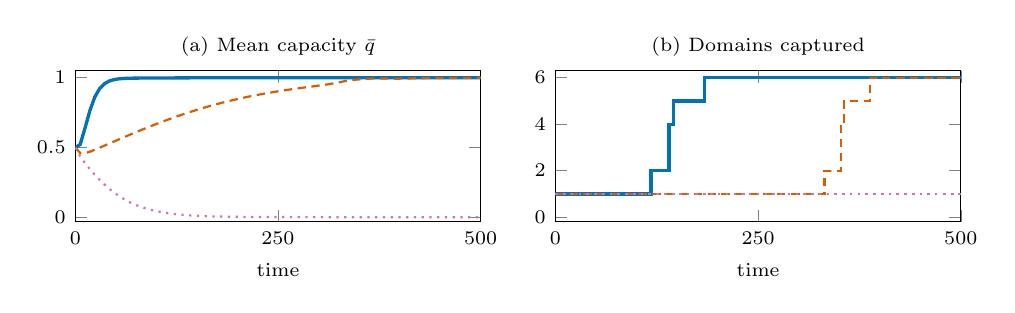
\begin{tikzpicture}
\begin{groupplot}[group style={group size=2 by 1, horizontal sep=0.95cm}, width=0.555\columnwidth, height=3.5cm,
  xmin=0, xmax=500, xtick={0,250,500}, tick label style={font=\scriptsize}, label style={font=\scriptsize},
  title style={font=\scriptsize, yshift=-1ex}, xlabel={time}]
\nextgroupplot[title={(a) Mean capacity $\bar q$}, ymin=-0.03, ymax=1.05, ytick={0,0.5,1}]
\addplot[cD, very thick] coordinates {(0,0.5000) (6,0.5230) (12,0.6403) (18,0.7656) (24,0.8613) (30,0.9223) (36,0.9575) (42,0.9767) (48,0.9869) (54,0.9922) (60,0.9949) (66,0.9963) (72,0.9970) (78,0.9974) (84,0.9976) (90,0.9977) (96,0.9978) (102,0.9980) (108,0.9981) (114,0.9984) (120,0.9986) (126,0.9988) (132,0.9989) (138,0.9991) (144,0.9993) (150,0.9994) (156,0.9995) (162,0.9995) (168,0.9994) (174,0.9994) (180,0.9994) (186,0.9995) (192,0.9995) (198,0.9996) (204,0.9997) (210,0.9997) (216,0.9998) (222,0.9998) (228,0.9998) (234,0.9998) (240,0.9998) (246,0.9998) (252,0.9998) (258,0.9998) (264,0.9998) (270,0.9998) (276,0.9998) (282,0.9998) (288,0.9998) (294,0.9998) (300,0.9998) (306,0.9998) (312,0.9998) (318,0.9998) (324,0.9998) (330,0.9998) (336,0.9998) (342,0.9998) (348,0.9998) (354,0.9998) (360,0.9998) (366,0.9998) (372,0.9998) (378,0.9998) (384,0.9998) (390,0.9998) (396,0.9998) (402,0.9998) (408,0.9998) (414,0.9998) (420,0.9998) (426,0.9998) (432,0.9998) (438,0.9998) (444,0.9998) (450,0.9998) (456,0.9998) (462,0.9998) (468,0.9998) (474,0.9998) (480,0.9998) (486,0.9998) (492,0.9998) (498,0.9998) (500,0.9998)};
\label{pl:chi08}
\addplot[cE, thick, densely dashed] coordinates {(0,0.5000) (6,0.4623) (12,0.4609) (18,0.4711) (24,0.4848) (30,0.4996) (36,0.5146) (42,0.5297) (48,0.5448) (54,0.5598) (60,0.5747) (66,0.5894) (72,0.6040) (78,0.6184) (84,0.6326) (90,0.6466) (96,0.6603) (102,0.6738) (108,0.6870) (114,0.6999) (120,0.7125) (126,0.7247) (132,0.7367) (138,0.7482) (144,0.7595) (150,0.7704) (156,0.7809) (162,0.7911) (168,0.8010) (174,0.8105) (180,0.8196) (186,0.8284) (192,0.8369) (198,0.8450) (204,0.8528) (210,0.8603) (216,0.8675) (222,0.8743) (228,0.8809) (234,0.8872) (240,0.8933) (246,0.8991) (252,0.9047) (258,0.9100) (264,0.9151) (270,0.9201) (276,0.9249) (282,0.9296) (288,0.9342) (294,0.9388) (300,0.9434) (306,0.9482) (312,0.9532) (318,0.9589) (324,0.9654) (330,0.9728) (336,0.9796) (342,0.9841) (348,0.9871) (354,0.9898) (360,0.9923) (366,0.9940) (372,0.9947) (378,0.9945) (384,0.9938) (390,0.9932) (396,0.9931) (402,0.9936) (408,0.9943) (414,0.9952) (420,0.9959) (426,0.9965) (432,0.9971) (438,0.9975) (444,0.9978) (450,0.9981) (456,0.9984) (462,0.9986) (468,0.9987) (474,0.9988) (480,0.9989) (486,0.9990) (492,0.9991) (498,0.9991) (500,0.9992)};
\label{pl:chi03}
\addplot[cF, thick, dotted] coordinates {(0,0.5000) (6,0.4382) (12,0.3894) (18,0.3463) (24,0.3066) (30,0.2699) (36,0.2363) (42,0.2057) (48,0.1783) (54,0.1538) (60,0.1323) (66,0.1134) (72,0.0970) (78,0.0828) (84,0.0706) (90,0.0601) (96,0.0512) (102,0.0436) (108,0.0372) (114,0.0318) (120,0.0272) (126,0.0233) (132,0.0200) (138,0.0173) (144,0.0150) (150,0.0131) (156,0.0115) (162,0.0101) (168,0.0090) (174,0.0080) (180,0.0072) (186,0.0066) (192,0.0060) (198,0.0055) (204,0.0051) (210,0.0048) (216,0.0045) (222,0.0043) (228,0.0041) (234,0.0040) (240,0.0038) (246,0.0037) (252,0.0036) (258,0.0036) (264,0.0035) (270,0.0034) (276,0.0034) (282,0.0034) (288,0.0033) (294,0.0033) (300,0.0033) (306,0.0033) (312,0.0032) (318,0.0032) (324,0.0032) (330,0.0032) (336,0.0032) (342,0.0032) (348,0.0032) (354,0.0032) (360,0.0032) (366,0.0032) (372,0.0032) (378,0.0032) (384,0.0032) (390,0.0032) (396,0.0032) (402,0.0032) (408,0.0032) (414,0.0032) (420,0.0032) (426,0.0032) (432,0.0032) (438,0.0032) (444,0.0032) (450,0.0032) (456,0.0032) (462,0.0032) (468,0.0032) (474,0.0032) (480,0.0032) (486,0.0032) (492,0.0032) (498,0.0032) (500,0.0032)};
\label{pl:chi01}
\nextgroupplot[title={(b) Domains captured}, ymin=-0.2, ymax=6.3, ytick={0,2,4,6}]
\addplot[cD, very thick, const plot] coordinates {(0,1.0000) (2,1.0000) (4,1.0000) (6,1.0000) (8,1.0000) (10,1.0000) (12,1.0000) (14,1.0000) (16,1.0000) (18,1.0000) (20,1.0000) (22,1.0000) (24,1.0000) (26,1.0000) (28,1.0000) (30,1.0000) (32,1.0000) (34,1.0000) (36,1.0000) (38,1.0000) (40,1.0000) (42,1.0000) (44,1.0000) (46,1.0000) (48,1.0000) (50,1.0000) (52,1.0000) (54,1.0000) (56,1.0000) (58,1.0000) (60,1.0000) (62,1.0000) (64,1.0000) (66,1.0000) (68,1.0000) (70,1.0000) (72,1.0000) (74,1.0000) (76,1.0000) (78,1.0000) (80,1.0000) (82,1.0000) (84,1.0000) (86,1.0000) (88,1.0000) (90,1.0000) (92,1.0000) (94,1.0000) (96,1.0000) (98,1.0000) (100,1.0000) (102,1.0000) (104,1.0000) (106,1.0000) (108,1.0000) (110,1.0000) (112,1.0000) (114,1.0000) (116,1.0000) (118,2.0000) (120,2.0000) (122,2.0000) (124,2.0000) (126,2.0000) (128,2.0000) (130,2.0000) (132,2.0000) (134,2.0000) (136,2.0000) (138,2.0000) (140,4.0000) (142,4.0000) (144,4.0000) (146,5.0000) (148,5.0000) (150,5.0000) (152,5.0000) (154,5.0000) (156,5.0000) (158,5.0000) (160,5.0000) (162,5.0000) (164,5.0000) (166,5.0000) (168,5.0000) (170,5.0000) (172,5.0000) (174,5.0000) (176,5.0000) (178,5.0000) (180,5.0000) (182,5.0000) (184,6.0000) (186,6.0000) (188,6.0000) (190,6.0000) (192,6.0000) (194,6.0000) (196,6.0000) (198,6.0000) (200,6.0000) (202,6.0000) (204,6.0000) (206,6.0000) (208,6.0000) (210,6.0000) (212,6.0000) (214,6.0000) (216,6.0000) (218,6.0000) (220,6.0000) (222,6.0000) (224,6.0000) (226,6.0000) (228,6.0000) (230,6.0000) (232,6.0000) (234,6.0000) (236,6.0000) (238,6.0000) (240,6.0000) (242,6.0000) (244,6.0000) (246,6.0000) (248,6.0000) (250,6.0000) (252,6.0000) (254,6.0000) (256,6.0000) (258,6.0000) (260,6.0000) (262,6.0000) (264,6.0000) (266,6.0000) (268,6.0000) (270,6.0000) (272,6.0000) (274,6.0000) (276,6.0000) (278,6.0000) (280,6.0000) (282,6.0000) (284,6.0000) (286,6.0000) (288,6.0000) (290,6.0000) (292,6.0000) (294,6.0000) (296,6.0000) (298,6.0000) (300,6.0000) (302,6.0000) (304,6.0000) (306,6.0000) (308,6.0000) (310,6.0000) (312,6.0000) (314,6.0000) (316,6.0000) (318,6.0000) (320,6.0000) (322,6.0000) (324,6.0000) (326,6.0000) (328,6.0000) (330,6.0000) (332,6.0000) (334,6.0000) (336,6.0000) (338,6.0000) (340,6.0000) (342,6.0000) (344,6.0000) (346,6.0000) (348,6.0000) (350,6.0000) (352,6.0000) (354,6.0000) (356,6.0000) (358,6.0000) (360,6.0000) (362,6.0000) (364,6.0000) (366,6.0000) (368,6.0000) (370,6.0000) (372,6.0000) (374,6.0000) (376,6.0000) (378,6.0000) (380,6.0000) (382,6.0000) (384,6.0000) (386,6.0000) (388,6.0000) (390,6.0000) (392,6.0000) (394,6.0000) (396,6.0000) (398,6.0000) (400,6.0000) (402,6.0000) (404,6.0000) (406,6.0000) (408,6.0000) (410,6.0000) (412,6.0000) (414,6.0000) (416,6.0000) (418,6.0000) (420,6.0000) (422,6.0000) (424,6.0000) (426,6.0000) (428,6.0000) (430,6.0000) (432,6.0000) (434,6.0000) (436,6.0000) (438,6.0000) (440,6.0000) (442,6.0000) (444,6.0000) (446,6.0000) (448,6.0000) (450,6.0000) (452,6.0000) (454,6.0000) (456,6.0000) (458,6.0000) (460,6.0000) (462,6.0000) (464,6.0000) (466,6.0000) (468,6.0000) (470,6.0000) (472,6.0000) (474,6.0000) (476,6.0000) (478,6.0000) (480,6.0000) (482,6.0000) (484,6.0000) (486,6.0000) (488,6.0000) (490,6.0000) (492,6.0000) (494,6.0000) (496,6.0000) (498,6.0000) (500,6.0000)};
\addplot[cE, thick, densely dashed, const plot] coordinates {(0,1.0000) (2,1.0000) (4,1.0000) (6,1.0000) (8,1.0000) (10,1.0000) (12,1.0000) (14,1.0000) (16,1.0000) (18,1.0000) (20,1.0000) (22,1.0000) (24,1.0000) (26,1.0000) (28,1.0000) (30,1.0000) (32,1.0000) (34,1.0000) (36,1.0000) (38,1.0000) (40,1.0000) (42,1.0000) (44,1.0000) (46,1.0000) (48,1.0000) (50,1.0000) (52,1.0000) (54,1.0000) (56,1.0000) (58,1.0000) (60,1.0000) (62,1.0000) (64,1.0000) (66,1.0000) (68,1.0000) (70,1.0000) (72,1.0000) (74,1.0000) (76,1.0000) (78,1.0000) (80,1.0000) (82,1.0000) (84,1.0000) (86,1.0000) (88,1.0000) (90,1.0000) (92,1.0000) (94,1.0000) (96,1.0000) (98,1.0000) (100,1.0000) (102,1.0000) (104,1.0000) (106,1.0000) (108,1.0000) (110,1.0000) (112,1.0000) (114,1.0000) (116,1.0000) (118,1.0000) (120,1.0000) (122,1.0000) (124,1.0000) (126,1.0000) (128,1.0000) (130,1.0000) (132,1.0000) (134,1.0000) (136,1.0000) (138,1.0000) (140,1.0000) (142,1.0000) (144,1.0000) (146,1.0000) (148,1.0000) (150,1.0000) (152,1.0000) (154,1.0000) (156,1.0000) (158,1.0000) (160,1.0000) (162,1.0000) (164,1.0000) (166,1.0000) (168,1.0000) (170,1.0000) (172,1.0000) (174,1.0000) (176,1.0000) (178,1.0000) (180,1.0000) (182,1.0000) (184,1.0000) (186,1.0000) (188,1.0000) (190,1.0000) (192,1.0000) (194,1.0000) (196,1.0000) (198,1.0000) (200,1.0000) (202,1.0000) (204,1.0000) (206,1.0000) (208,1.0000) (210,1.0000) (212,1.0000) (214,1.0000) (216,1.0000) (218,1.0000) (220,1.0000) (222,1.0000) (224,1.0000) (226,1.0000) (228,1.0000) (230,1.0000) (232,1.0000) (234,1.0000) (236,1.0000) (238,1.0000) (240,1.0000) (242,1.0000) (244,1.0000) (246,1.0000) (248,1.0000) (250,1.0000) (252,1.0000) (254,1.0000) (256,1.0000) (258,1.0000) (260,1.0000) (262,1.0000) (264,1.0000) (266,1.0000) (268,1.0000) (270,1.0000) (272,1.0000) (274,1.0000) (276,1.0000) (278,1.0000) (280,1.0000) (282,1.0000) (284,1.0000) (286,1.0000) (288,1.0000) (290,1.0000) (292,1.0000) (294,1.0000) (296,1.0000) (298,1.0000) (300,1.0000) (302,1.0000) (304,1.0000) (306,1.0000) (308,1.0000) (310,1.0000) (312,1.0000) (314,1.0000) (316,1.0000) (318,1.0000) (320,1.0000) (322,1.0000) (324,1.0000) (326,1.0000) (328,1.0000) (330,1.0000) (332,2.0000) (334,2.0000) (336,2.0000) (338,2.0000) (340,2.0000) (342,2.0000) (344,2.0000) (346,2.0000) (348,2.0000) (350,2.0000) (352,4.0000) (354,4.0000) (356,5.0000) (358,5.0000) (360,5.0000) (362,5.0000) (364,5.0000) (366,5.0000) (368,5.0000) (370,5.0000) (372,5.0000) (374,5.0000) (376,5.0000) (378,5.0000) (380,5.0000) (382,5.0000) (384,5.0000) (386,5.0000) (388,6.0000) (390,6.0000) (392,6.0000) (394,6.0000) (396,6.0000) (398,6.0000) (400,6.0000) (402,6.0000) (404,6.0000) (406,6.0000) (408,6.0000) (410,6.0000) (412,6.0000) (414,6.0000) (416,6.0000) (418,6.0000) (420,6.0000) (422,6.0000) (424,6.0000) (426,6.0000) (428,6.0000) (430,6.0000) (432,6.0000) (434,6.0000) (436,6.0000) (438,6.0000) (440,6.0000) (442,6.0000) (444,6.0000) (446,6.0000) (448,6.0000) (450,6.0000) (452,6.0000) (454,6.0000) (456,6.0000) (458,6.0000) (460,6.0000) (462,6.0000) (464,6.0000) (466,6.0000) (468,6.0000) (470,6.0000) (472,6.0000) (474,6.0000) (476,6.0000) (478,6.0000) (480,6.0000) (482,6.0000) (484,6.0000) (486,6.0000) (488,6.0000) (490,6.0000) (492,6.0000) (494,6.0000) (496,6.0000) (498,6.0000) (500,6.0000)};
\addplot[cF, thick, dotted, const plot] coordinates {(0,1.0000) (2,1.0000) (4,1.0000) (6,1.0000) (8,1.0000) (10,1.0000) (12,1.0000) (14,1.0000) (16,1.0000) (18,1.0000) (20,1.0000) (22,1.0000) (24,1.0000) (26,1.0000) (28,1.0000) (30,1.0000) (32,1.0000) (34,1.0000) (36,1.0000) (38,1.0000) (40,1.0000) (42,1.0000) (44,1.0000) (46,1.0000) (48,1.0000) (50,1.0000) (52,1.0000) (54,1.0000) (56,1.0000) (58,1.0000) (60,1.0000) (62,1.0000) (64,1.0000) (66,1.0000) (68,1.0000) (70,1.0000) (72,1.0000) (74,1.0000) (76,1.0000) (78,1.0000) (80,1.0000) (82,1.0000) (84,1.0000) (86,1.0000) (88,1.0000) (90,1.0000) (92,1.0000) (94,1.0000) (96,1.0000) (98,1.0000) (100,1.0000) (102,1.0000) (104,1.0000) (106,1.0000) (108,1.0000) (110,1.0000) (112,1.0000) (114,1.0000) (116,1.0000) (118,1.0000) (120,1.0000) (122,1.0000) (124,1.0000) (126,1.0000) (128,1.0000) (130,1.0000) (132,1.0000) (134,1.0000) (136,1.0000) (138,1.0000) (140,1.0000) (142,1.0000) (144,1.0000) (146,1.0000) (148,1.0000) (150,1.0000) (152,1.0000) (154,1.0000) (156,1.0000) (158,1.0000) (160,1.0000) (162,1.0000) (164,1.0000) (166,1.0000) (168,1.0000) (170,1.0000) (172,1.0000) (174,1.0000) (176,1.0000) (178,1.0000) (180,1.0000) (182,1.0000) (184,1.0000) (186,1.0000) (188,1.0000) (190,1.0000) (192,1.0000) (194,1.0000) (196,1.0000) (198,1.0000) (200,1.0000) (202,1.0000) (204,1.0000) (206,1.0000) (208,1.0000) (210,1.0000) (212,1.0000) (214,1.0000) (216,1.0000) (218,1.0000) (220,1.0000) (222,1.0000) (224,1.0000) (226,1.0000) (228,1.0000) (230,1.0000) (232,1.0000) (234,1.0000) (236,1.0000) (238,1.0000) (240,1.0000) (242,1.0000) (244,1.0000) (246,1.0000) (248,1.0000) (250,1.0000) (252,1.0000) (254,1.0000) (256,1.0000) (258,1.0000) (260,1.0000) (262,1.0000) (264,1.0000) (266,1.0000) (268,1.0000) (270,1.0000) (272,1.0000) (274,1.0000) (276,1.0000) (278,1.0000) (280,1.0000) (282,1.0000) (284,1.0000) (286,1.0000) (288,1.0000) (290,1.0000) (292,1.0000) (294,1.0000) (296,1.0000) (298,1.0000) (300,1.0000) (302,1.0000) (304,1.0000) (306,1.0000) (308,1.0000) (310,1.0000) (312,1.0000) (314,1.0000) (316,1.0000) (318,1.0000) (320,1.0000) (322,1.0000) (324,1.0000) (326,1.0000) (328,1.0000) (330,1.0000) (332,1.0000) (334,1.0000) (336,1.0000) (338,1.0000) (340,1.0000) (342,1.0000) (344,1.0000) (346,1.0000) (348,1.0000) (350,1.0000) (352,1.0000) (354,1.0000) (356,1.0000) (358,1.0000) (360,1.0000) (362,1.0000) (364,1.0000) (366,1.0000) (368,1.0000) (370,1.0000) (372,1.0000) (374,1.0000) (376,1.0000) (378,1.0000) (380,1.0000) (382,1.0000) (384,1.0000) (386,1.0000) (388,1.0000) (390,1.0000) (392,1.0000) (394,1.0000) (396,1.0000) (398,1.0000) (400,1.0000) (402,1.0000) (404,1.0000) (406,1.0000) (408,1.0000) (410,1.0000) (412,1.0000) (414,1.0000) (416,1.0000) (418,1.0000) (420,1.0000) (422,1.0000) (424,1.0000) (426,1.0000) (428,1.0000) (430,1.0000) (432,1.0000) (434,1.0000) (436,1.0000) (438,1.0000) (440,1.0000) (442,1.0000) (444,1.0000) (446,1.0000) (448,1.0000) (450,1.0000) (452,1.0000) (454,1.0000) (456,1.0000) (458,1.0000) (460,1.0000) (462,1.0000) (464,1.0000) (466,1.0000) (468,1.0000) (470,1.0000) (472,1.0000) (474,1.0000) (476,1.0000) (478,1.0000) (480,1.0000) (482,1.0000) (484,1.0000) (486,1.0000) (488,1.0000) (490,1.0000) (492,1.0000) (494,1.0000) (496,1.0000) (498,1.0000) (500,1.0000)};
\end{groupplot}
\end{tikzpicture}

\caption{Selection on conversion capacity in the six-domain field of Section~\ref{sec:field} at $\theta=0.6$, where capture from development stays there. Two carrier types differ only in capacity, $q\in\{0,1\}$. Appropriability $\chi=0.8$ (\ref{pl:chi08}), $0.3$ (\ref{pl:chi03}), $0.1$ (\ref{pl:chi01}). (a)~Practice-weighted mean capacity. (b)~Domains with $x_i>0.5$.}
\label{fig:capacity}
\end{figure}

\paragraph{Illustration.} Figure~\ref{fig:capacity} uses the six-domain field of Section~\ref{sec:field} with conversion $\theta=0.6$ from development, where capture launched from development stays there. A unit of capacity adds conversion $0.5$ from development into each other domain (smaller amounts elsewhere; Appendix~\ref{app:numerics}) at cost $0.05$ per decision. With $\chi=0.8$ mean capacity passes $0.9$ at $t\approx28$; cultivated coupling then exceeds the cascade threshold, and every domain is captured by $t\approx184$. With $\chi=0.3$, just above the value $0.25$ at which capacity starts to pay in development, the same happens more slowly. With $\chi=0.1$ the high-capacity type is displaced and capture stays in development. The runs differ in nothing but appropriability, and freezing capacity at its initial mean also leaves capture in development. Once the field is captured, the net advantage of capacity in development is five times its initial value ($0.51$ against $0.10$ at $\chi=0.8$): capture raises the return to control.

\section{Audit and Reform in Coupled Fields}\label{sec:field}

\begin{proposition}[Certificates]\label{prop:cert}
Let $\mu=0$. (a) Isolated tests cannot certify: for any $n\ge2$ and diagonal values $R_{ii}<1$, there are conversions under which full capture is stable and is the only stable configuration containing a given domain. (b) A row certifies its domain: if $\sum_jR_{ij}<1$, then $x_i\to0$ from every state with $x_i(0)<1$, whatever happens elsewhere. (c) The core is exact: if $\core(N)=\emptyset$, no capture attracts every state with all shares below one; otherwise, barring ties $s_k=1$ in the pruning, $Z_{\core(N)}$ is stable and contains every stable configuration. (d) A selector can be firewalled robustly: if row $\dE$ sums to less than one, evaluation stays uncaptured whatever is captured elsewhere.
\end{proposition}

Part (a) is a field-level fallacy of composition; (b)--(d) make it constructive. An authority that measures all inbound channels of its own domain can certify that domain conservatively. What requires joint assessment is the sharp test (c), which domains lie in the hull of a given seed, and which are keystones.

\begin{proposition}[Cascades, reforms and keystones]\label{prop:reform}
Let $\mu=0$. (i) If $x_j\to1$ for all $j$ in a seed $\cS_0$, then $x_i\to1$ for every $i\in\hull(\cS_0)$. (ii) Start in the basin of a stable $Z_\cC$ with every share in $(0,1)$, and let a sustained reform drive $x_i\to0$ for each $i$ in $\cQ\subseteq\cC$, by holding the share at zero or by a margin reform (raising $c_i$ or $d_i$, lowering $a_i$, or cutting inbound $b_{ij}$) that makes the reformed $s_i(\cC)<1$. Then $x_k\to0$ for every $k$ outside $\core(\cC\setminus\cQ)$. A margin reform that leaves the reformed $s_i(\cC)>1$ is re-absorbed from states near $Z_\cC$. (iii) After a reform, a domain is recaptured if it is re-seeded and its inbound conversion from the set still captured exceeds one; a reform that resets a domain's state or own conversion without lowering that inbound conversion is re-absorbed.
\end{proposition}

Call $\cQ\subseteq\cC$ a \emph{keystone set} of $Z_\cC$ if $\core(\cC\setminus\cQ)\neq\cC\setminus\cQ$: reforming $\cQ$ takes down further domains. Finding a minimum keystone set is the collapsed $k$-core problem, NP-hard in general \citep{zhang2017collapsed,bhawalkar2015} and trivial by enumeration for the dozen or so domains of a real field. The stability conditions of $Z_\cC$ involve only the rows indexed by $\cC$ and the inbound conversion of outside domains from $\cC$, so a mutually sustaining set stays locally stable whatever the outbound conversion of the domain where the practice began: a way of succeeding can outlive its origin.

\paragraph{Illustration.} Development is self-sustaining ($R_{\dD\dD}=1.3$); every other domain is subcritical alone ($R_{ii}=0.3$), with mutual conversion $\varphi=0.11$ and conversion $\theta$ from development; entry is $\mu=10^{-4}$ (Appendix~\ref{app:numerics}). At $\theta=0.6$, capture launched from development stays there, yet many configurations are stable, including three that capture both selector domains without full capture and survive the entry rate (Appendix~\ref{app:numerics}): general-purpose coupling changes which configuration a development seed reaches, not which can exist. At $\theta=1.2$ every domain lies in the hull of development. Procurement is captured at $t\approx43$, evaluation and information at $t\approx56$, standards at $t\approx67$ and formation at $t\approx106$ (Figure~\ref{fig:field}a). Cutting conversion from development into evaluation and formation to $0.2$ gives each a row sum of $0.94$, so by Proposition~\ref{prop:cert}(d) both stay independent whatever else is captured (Figure~\ref{fig:field}b). In the captured field, resetting standards is re-absorbed by $t\approx38$ (inbound conversion $1.64$); behind a firewall from development (inbound $0.64$) the same reform holds. Development is the keystone of full capture, since without it each other domain receives $0.74$. But a keystone can re-absorb its own reform: with feedback $\psi$ from each other domain into development, doubling $c_\dD$ unwinds the field only if $(1.3+5\psi)/2<1$, and at $\psi=0.15$ the field stays captured.

\section{Selecting the Selectors}\label{sec:selectors}

\paragraph{Harm that selection does not see.} Let the practice in development deplete a shared condition $V\in(0,K]$, such as the integrity of a critical service or independent research capacity:
\begin{equation}\label{eq:V}
\dot V=V\big[\rho(1-V/K)-hx_\dD\big].
\end{equation}
$V$ enters every practice's absolute payoff alike, so it cancels from relative payoffs: success within a selection process is distinct from contribution to its conditions. Under capture $V$ falls to $K(1-h/\rho)$ if $h<\rho$, a finite loss, and to zero if $h>\rho$; collapse, $V$ below a functional floor, can occur in either case.

\paragraph{Masking as a panel average.} Correction is triggered when the \emph{reported} condition falls to $\Valarm$. Let reports average over a panel of evaluators. A fraction $x_\dE$ of them shares the lineage of the evaluated practice (its training, funding or tooling) and reports the condition a fraction $\beta$ of the way toward full health; the rest report it accurately:
\begin{equation}\label{eq:y}
\tilde V=V+\beta x_\dE(K-V).
\end{equation}
Let $t_{\mathrm{det}}=\inf\{t:\tilde V(t)\le\Valarm\}$, with $\inf\emptyset=\infty$.

\begin{proposition}[Detection]\label{prop:detect}
(i) The alarm fires only once $V\le V_{\mathrm{eff}}(x_\dE)=(\Valarm-\beta x_\dE K)/(1-\beta x_\dE)$, which decreases in $x_\dE$ when $\beta>0$. (ii) If $\beta x_\dE(t)\ge\Valarm/K$ for all $t\ge t_1$ and the alarm has not fired by $t_1$, it never fires; strict silencing requires $\beta\ge\Valarm/K$. (iii) If $V$ reaches $\Valarm$ at $t_A$, then declines as $\dot V=-\lambda V$, and $x_\dE\ge\bar x$ thereafter, then
\[t_{\mathrm{det}}-t_A\ \ge\ \frac1\lambda\ln\frac{(1-\beta\bar x)\Valarm}{\Valarm-\beta\bar xK},\]
with equality when $x_\dE=\bar x$; the delay diverges as $\beta\bar x\uparrow\Valarm/K$.
\end{proposition}

Detection is not correction. After the alarm, deciding takes time $\tau_d$ and reversing takes time $\tau_r$, short for margin levers and long for levers that act through decaying rule stocks; $t_{\mathrm{det}}+\tau_d+\tau_r$ must precede the time at which uncorrected $V$ crosses the floor, a necessary but not sufficient condition. Faster cascades and faster harm shorten that window; neither shortens $\tau_d$, which institutions set.

\paragraph{Layers of closure.} Masking a measurement is the simplest form of epistemic closure. Others are distinct and need not form a ladder: \emph{interpretation} (the same evidence is read through a fixed frame), \emph{representation and agenda} (some consequences have no category in which to be recorded or raised), \emph{formation of preferences} (education, incentives and mediation change what seems worth pursuing) and \emph{authority to act} (known errors cannot move budgets, rules or behavior). In our equations measurement enters through $\beta$, formation through Remark~\ref{rem:formation} and authority through Remark~\ref{rem:mincut}; interpretation and representation remain verbal mechanisms here. A condition that has vanished from a system's categories has not vanished from the world. Nor is every change of preference capture, since learning and moral growth change preferences too; what matters is deception, unilateral control, and the absence of conditions for reflection and of alternatives.

\begin{remark}[Why the alarm cannot be recalibrated]\label{rem:indist}
If the panel's composition is unknown, a report $\tilde V$ is consistent with every true condition in $[\max\{0,(\tilde V-\beta K)/(1-\beta)\},\tilde V]$. Two states with the same report but disjoint safe actions cannot both be handled safely by any rule that acts on the report alone, however much computation it uses. Recalibration needs an independent channel; its gap from $\tilde V$ measures $\beta x_\dE(K-V)$ directly.
\end{remark}

\begin{remark}[Correction as a path]\label{rem:mincut}
Correction needs a path from the harm through observation, reporting and decision to an actor with authority to act. Group the nodes of this \emph{error-access graph} into control units, merging nodes that share funding, lineage, data or authority. Correction survives the capture of $k$ units only if the minimum cut over units exceeds $k$, and only if surviving paths deliver within the correction window. A hundred models trained on the same data count as one unit.
\end{remark}

\begin{remark}[Formation]\label{rem:formation}
Formation can enter in two further ways, both of which keep the system cooperative. If formation normalizes the practice so that its cost stops registering, $c_i(x_\dF)=c^0_i-g_ix_\dF$, captured formation multiplies every row it reaches by $c^0_i/(c^0_i-g_i)$, and if $g_i\ge c^0_i$ the practice holds domain $i$ with no rule support. If evaluators are formed on the practice's outputs, $\beta=\beta^0+\beta^1x_\dF$, and panels of mixed lineage stop restoring independence, because every lineage is formed on the same material.
\end{remark}

\begin{remark}[Dependence]\label{rem:dependence}
Power can help a practice succeed under given conditions, and it can set those conditions \citep{strange1988,lukes2005}. If degradation of $V$ deepens dependence on the practice's infrastructure, $b_{ij}(V)=b^0_{ij}+b^1_{ij}(1-V/K)$, inbound conversion rises as $V$ falls, and domain $i$ becomes capturable once $V<K\big(1-(1-s^0_i)/s^1_i\big)$ with no change in the practice, where $s^0_i,s^1_i$ sum the normalized $b^0,b^1$ over the captured set. Harm then feeds capture, much as dependence on network hubs converts into leverage over those who depend on them \citep{farrell2019}.
\end{remark}

\begin{figure*}[t]
\centering
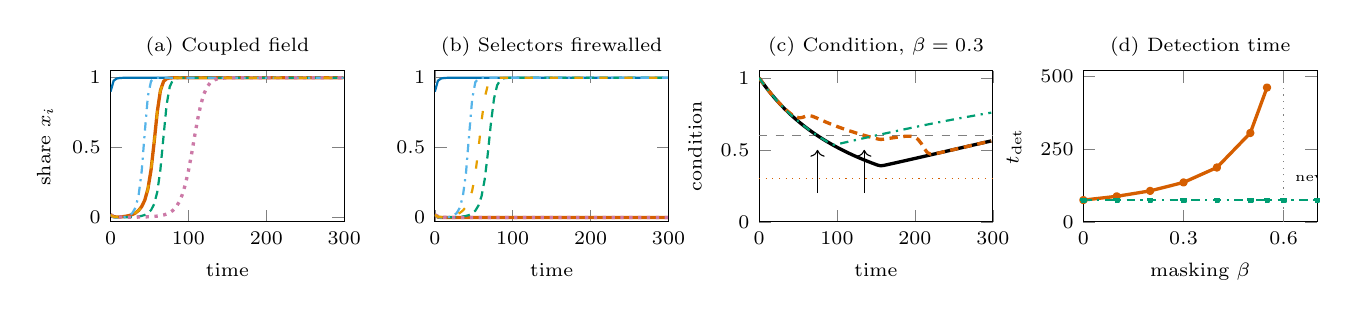
\begin{tikzpicture}
\begin{groupplot}[group style={group size=4 by 1, horizontal sep=1.15cm}, width=4.55cm, height=3.5cm,
  tick label style={font=\scriptsize}, label style={font=\scriptsize}, title style={font=\scriptsize, yshift=-1ex},
  every axis plot/.append style={line join=round}]
\nextgroupplot[title={(a) Coupled field}, xmin=0, xmax=300, ymin=-0.03, ymax=1.05, xtick={0,100,200,300}, ytick={0,0.5,1}, xlabel={time}, ylabel={share $x_i$}]
\addplot[cD, thick] coordinates {(0,0.9000) (4,0.9790) (8,0.9942) (12,0.9981) (16,0.9992) (20,0.9995) (24,0.9996) (28,0.9997) (32,0.9997) (36,0.9997) (40,0.9997) (44,0.9997) (48,0.9997) (52,0.9997) (56,0.9997) (60,0.9997) (64,0.9997) (68,0.9997) (72,0.9997) (76,0.9997) (80,0.9997) (84,0.9997) (88,0.9997) (92,0.9997) (96,0.9997) (100,0.9997) (104,0.9997) (108,0.9997) (112,0.9997) (116,0.9997) (120,0.9997) (124,0.9997) (128,0.9997) (132,0.9997) (136,0.9997) (140,0.9997) (144,0.9997) (148,0.9997) (152,0.9997) (156,0.9997) (160,0.9997) (164,0.9997) (168,0.9997) (172,0.9997) (176,0.9997) (180,0.9997) (184,0.9997) (188,0.9997) (192,0.9997) (196,0.9997) (200,0.9997) (204,0.9997) (208,0.9997) (212,0.9997) (216,0.9997) (220,0.9997) (224,0.9997) (228,0.9997) (232,0.9997) (236,0.9997) (240,0.9997) (244,0.9997) (248,0.9997) (252,0.9997) (256,0.9997) (260,0.9997) (264,0.9997) (268,0.9997) (272,0.9997) (276,0.9997) (280,0.9997) (284,0.9997) (288,0.9997) (292,0.9997) (296,0.9997) (299,0.9997)};
\label{pl:D}
\addplot[cE, very thick] coordinates {(0,0.0200) (4,0.0058) (8,0.0043) (12,0.0049) (16,0.0067) (20,0.0098) (24,0.0146) (28,0.0221) (32,0.0335) (36,0.0511) (40,0.0790) (44,0.1254) (48,0.2055) (52,0.3409) (56,0.5396) (60,0.7560) (64,0.9069) (68,0.9729) (72,0.9933) (76,0.9983) (80,0.9995) (84,0.9997) (88,0.9997) (92,0.9998) (96,0.9998) (100,0.9998) (104,0.9998) (108,0.9998) (112,0.9998) (116,0.9998) (120,0.9998) (124,0.9998) (128,0.9998) (132,0.9998) (136,0.9998) (140,0.9998) (144,0.9998) (148,0.9998) (152,0.9998) (156,0.9998) (160,0.9998) (164,0.9998) (168,0.9998) (172,0.9998) (176,0.9998) (180,0.9998) (184,0.9998) (188,0.9998) (192,0.9998) (196,0.9998) (200,0.9998) (204,0.9998) (208,0.9998) (212,0.9998) (216,0.9998) (220,0.9998) (224,0.9998) (228,0.9998) (232,0.9998) (236,0.9998) (240,0.9998) (244,0.9998) (248,0.9998) (252,0.9998) (256,0.9998) (260,0.9998) (264,0.9998) (268,0.9998) (272,0.9998) (276,0.9998) (280,0.9998) (284,0.9998) (288,0.9998) (292,0.9998) (296,0.9998) (299,0.9998)};
\label{pl:E}
\addplot[cS, thick, densely dashed] coordinates {(0,0.0200) (4,0.0043) (8,0.0019) (12,0.0015) (16,0.0016) (20,0.0019) (24,0.0026) (28,0.0037) (32,0.0054) (36,0.0081) (40,0.0122) (44,0.0190) (48,0.0310) (52,0.0534) (56,0.0970) (60,0.1830) (64,0.3426) (68,0.5795) (72,0.8075) (76,0.9362) (80,0.9829) (84,0.9958) (88,0.9989) (92,0.9996) (96,0.9997) (100,0.9998) (104,0.9998) (108,0.9998) (112,0.9998) (116,0.9998) (120,0.9998) (124,0.9998) (128,0.9998) (132,0.9998) (136,0.9998) (140,0.9998) (144,0.9998) (148,0.9998) (152,0.9998) (156,0.9998) (160,0.9998) (164,0.9998) (168,0.9998) (172,0.9998) (176,0.9998) (180,0.9998) (184,0.9998) (188,0.9998) (192,0.9998) (196,0.9998) (200,0.9998) (204,0.9998) (208,0.9998) (212,0.9998) (216,0.9998) (220,0.9998) (224,0.9998) (228,0.9998) (232,0.9998) (236,0.9998) (240,0.9998) (244,0.9998) (248,0.9998) (252,0.9998) (256,0.9998) (260,0.9998) (264,0.9998) (268,0.9998) (272,0.9998) (276,0.9998) (280,0.9998) (284,0.9998) (288,0.9998) (292,0.9998) (296,0.9998) (299,0.9998)};
\label{pl:S}
\addplot[cP, thick, dashdotted] coordinates {(0,0.0200) (4,0.0017) (8,0.0011) (12,0.0016) (16,0.0031) (20,0.0066) (24,0.0145) (28,0.0320) (32,0.0712) (36,0.1572) (40,0.3323) (44,0.6138) (48,0.8710) (52,0.9754) (56,0.9967) (60,0.9995) (64,0.9998) (68,0.9999) (72,0.9999) (76,0.9999) (80,0.9999) (84,0.9999) (88,0.9999) (92,0.9999) (96,0.9999) (100,0.9999) (104,0.9999) (108,0.9999) (112,0.9999) (116,0.9999) (120,0.9999) (124,0.9999) (128,0.9999) (132,0.9999) (136,0.9999) (140,0.9999) (144,0.9999) (148,0.9999) (152,0.9999) (156,0.9999) (160,0.9999) (164,0.9999) (168,0.9999) (172,0.9999) (176,0.9999) (180,0.9999) (184,0.9999) (188,0.9999) (192,0.9999) (196,0.9999) (200,0.9999) (204,0.9999) (208,0.9999) (212,0.9999) (216,0.9999) (220,0.9999) (224,0.9999) (228,0.9999) (232,0.9999) (236,0.9999) (240,0.9999) (244,0.9999) (248,0.9999) (252,0.9999) (256,0.9999) (260,0.9999) (264,0.9999) (268,0.9999) (272,0.9999) (276,0.9999) (280,0.9999) (284,0.9999) (288,0.9999) (292,0.9999) (296,0.9999) (299,0.9999)};
\label{pl:P}
\addplot[cF, very thick, dotted] coordinates {(0,0.0200) (4,0.0102) (8,0.0061) (12,0.0043) (16,0.0035) (20,0.0031) (24,0.0030) (28,0.0031) (32,0.0033) (36,0.0037) (40,0.0042) (44,0.0048) (48,0.0057) (52,0.0068) (56,0.0084) (60,0.0106) (64,0.0138) (68,0.0184) (72,0.0253) (76,0.0356) (80,0.0513) (84,0.0751) (88,0.1107) (92,0.1628) (96,0.2364) (100,0.3343) (104,0.4537) (108,0.5838) (112,0.7079) (116,0.8108) (120,0.8859) (124,0.9349) (128,0.9643) (132,0.9809) (136,0.9899) (140,0.9946) (144,0.9970) (148,0.9983) (152,0.9989) (156,0.9992) (160,0.9993) (164,0.9994) (168,0.9994) (172,0.9994) (176,0.9995) (180,0.9995) (184,0.9995) (188,0.9995) (192,0.9995) (196,0.9995) (200,0.9995) (204,0.9995) (208,0.9995) (212,0.9995) (216,0.9995) (220,0.9995) (224,0.9995) (228,0.9995) (232,0.9995) (236,0.9995) (240,0.9995) (244,0.9995) (248,0.9995) (252,0.9995) (256,0.9995) (260,0.9995) (264,0.9995) (268,0.9995) (272,0.9995) (276,0.9995) (280,0.9995) (284,0.9995) (288,0.9995) (292,0.9995) (296,0.9995) (299,0.9995)};
\label{pl:F}
\addplot[cI, thick, loosely dashed] coordinates {(0,0.0200) (4,0.0058) (8,0.0043) (12,0.0049) (16,0.0067) (20,0.0098) (24,0.0146) (28,0.0221) (32,0.0335) (36,0.0511) (40,0.0790) (44,0.1254) (48,0.2055) (52,0.3409) (56,0.5396) (60,0.7560) (64,0.9069) (68,0.9729) (72,0.9933) (76,0.9983) (80,0.9995) (84,0.9997) (88,0.9997) (92,0.9998) (96,0.9998) (100,0.9998) (104,0.9998) (108,0.9998) (112,0.9998) (116,0.9998) (120,0.9998) (124,0.9998) (128,0.9998) (132,0.9998) (136,0.9998) (140,0.9998) (144,0.9998) (148,0.9998) (152,0.9998) (156,0.9998) (160,0.9998) (164,0.9998) (168,0.9998) (172,0.9998) (176,0.9998) (180,0.9998) (184,0.9998) (188,0.9998) (192,0.9998) (196,0.9998) (200,0.9998) (204,0.9998) (208,0.9998) (212,0.9998) (216,0.9998) (220,0.9998) (224,0.9998) (228,0.9998) (232,0.9998) (236,0.9998) (240,0.9998) (244,0.9998) (248,0.9998) (252,0.9998) (256,0.9998) (260,0.9998) (264,0.9998) (268,0.9998) (272,0.9998) (276,0.9998) (280,0.9998) (284,0.9998) (288,0.9998) (292,0.9998) (296,0.9998) (299,0.9998)};
\label{pl:I}
\nextgroupplot[title={(b) Selectors firewalled}, xmin=0, xmax=300, ymin=-0.03, ymax=1.05, xtick={0,100,200,300}, ytick={0,0.5,1}, xlabel={time}]
\addplot[cD, thick] coordinates {(0,0.9000) (4,0.9790) (8,0.9942) (12,0.9981) (16,0.9992) (20,0.9995) (24,0.9996) (28,0.9997) (32,0.9997) (36,0.9997) (40,0.9997) (44,0.9997) (48,0.9997) (52,0.9997) (56,0.9997) (60,0.9997) (64,0.9997) (68,0.9997) (72,0.9997) (76,0.9997) (80,0.9997) (84,0.9997) (88,0.9997) (92,0.9997) (96,0.9997) (100,0.9997) (104,0.9997) (108,0.9997) (112,0.9997) (116,0.9997) (120,0.9997) (124,0.9997) (128,0.9997) (132,0.9997) (136,0.9997) (140,0.9997) (144,0.9997) (148,0.9997) (152,0.9997) (156,0.9997) (160,0.9997) (164,0.9997) (168,0.9997) (172,0.9997) (176,0.9997) (180,0.9997) (184,0.9997) (188,0.9997) (192,0.9997) (196,0.9997) (200,0.9997) (204,0.9997) (208,0.9997) (212,0.9997) (216,0.9997) (220,0.9997) (224,0.9997) (228,0.9997) (232,0.9997) (236,0.9997) (240,0.9997) (244,0.9997) (248,0.9997) (252,0.9997) (256,0.9997) (260,0.9997) (264,0.9997) (268,0.9997) (272,0.9997) (276,0.9997) (280,0.9997) (284,0.9997) (288,0.9997) (292,0.9997) (296,0.9997) (299,0.9997)};
\addplot[cE, very thick] coordinates {(0,0.0200) (4,0.0033) (8,0.0008) (12,0.0003) (16,0.0003) (20,0.0003) (24,0.0003) (28,0.0003) (32,0.0003) (36,0.0003) (40,0.0003) (44,0.0003) (48,0.0003) (52,0.0003) (56,0.0003) (60,0.0003) (64,0.0003) (68,0.0003) (72,0.0004) (76,0.0004) (80,0.0004) (84,0.0004) (88,0.0004) (92,0.0004) (96,0.0004) (100,0.0004) (104,0.0004) (108,0.0004) (112,0.0004) (116,0.0004) (120,0.0004) (124,0.0004) (128,0.0004) (132,0.0004) (136,0.0004) (140,0.0004) (144,0.0004) (148,0.0004) (152,0.0004) (156,0.0004) (160,0.0004) (164,0.0004) (168,0.0004) (172,0.0004) (176,0.0004) (180,0.0004) (184,0.0004) (188,0.0004) (192,0.0004) (196,0.0004) (200,0.0004) (204,0.0004) (208,0.0004) (212,0.0004) (216,0.0004) (220,0.0004) (224,0.0004) (228,0.0004) (232,0.0004) (236,0.0004) (240,0.0004) (244,0.0004) (248,0.0004) (252,0.0004) (256,0.0004) (260,0.0004) (264,0.0004) (268,0.0004) (272,0.0004) (276,0.0004) (280,0.0004) (284,0.0004) (288,0.0004) (292,0.0004) (296,0.0004) (299,0.0004)};
\addplot[cS, thick, densely dashed] coordinates {(0,0.0200) (4,0.0043) (8,0.0019) (12,0.0015) (16,0.0016) (20,0.0019) (24,0.0026) (28,0.0037) (32,0.0054) (36,0.0080) (40,0.0120) (44,0.0184) (48,0.0295) (52,0.0494) (56,0.0858) (60,0.1530) (64,0.2714) (68,0.4550) (72,0.6736) (76,0.8506) (80,0.9458) (84,0.9831) (88,0.9951) (92,0.9985) (96,0.9994) (100,0.9996) (104,0.9997) (108,0.9997) (112,0.9997) (116,0.9997) (120,0.9997) (124,0.9997) (128,0.9997) (132,0.9997) (136,0.9997) (140,0.9997) (144,0.9997) (148,0.9997) (152,0.9997) (156,0.9997) (160,0.9997) (164,0.9997) (168,0.9997) (172,0.9997) (176,0.9997) (180,0.9997) (184,0.9997) (188,0.9997) (192,0.9997) (196,0.9997) (200,0.9997) (204,0.9997) (208,0.9997) (212,0.9997) (216,0.9997) (220,0.9997) (224,0.9997) (228,0.9997) (232,0.9997) (236,0.9997) (240,0.9997) (244,0.9997) (248,0.9997) (252,0.9997) (256,0.9997) (260,0.9997) (264,0.9997) (268,0.9997) (272,0.9997) (276,0.9997) (280,0.9997) (284,0.9997) (288,0.9997) (292,0.9997) (296,0.9997) (299,0.9997)};
\addplot[cP, thick, dashdotted] coordinates {(0,0.0200) (4,0.0017) (8,0.0011) (12,0.0016) (16,0.0031) (20,0.0066) (24,0.0143) (28,0.0315) (32,0.0695) (36,0.1519) (40,0.3181) (44,0.5880) (48,0.8498) (52,0.9678) (56,0.9950) (60,0.9992) (64,0.9998) (68,0.9998) (72,0.9998) (76,0.9998) (80,0.9999) (84,0.9999) (88,0.9999) (92,0.9999) (96,0.9999) (100,0.9999) (104,0.9999) (108,0.9999) (112,0.9999) (116,0.9999) (120,0.9999) (124,0.9999) (128,0.9999) (132,0.9999) (136,0.9999) (140,0.9999) (144,0.9999) (148,0.9999) (152,0.9999) (156,0.9999) (160,0.9999) (164,0.9999) (168,0.9999) (172,0.9999) (176,0.9999) (180,0.9999) (184,0.9999) (188,0.9999) (192,0.9999) (196,0.9999) (200,0.9999) (204,0.9999) (208,0.9999) (212,0.9999) (216,0.9999) (220,0.9999) (224,0.9999) (228,0.9999) (232,0.9999) (236,0.9999) (240,0.9999) (244,0.9999) (248,0.9999) (252,0.9999) (256,0.9999) (260,0.9999) (264,0.9999) (268,0.9999) (272,0.9999) (276,0.9999) (280,0.9999) (284,0.9999) (288,0.9999) (292,0.9999) (296,0.9999) (299,0.9999)};
\addplot[cF, very thick, dotted] coordinates {(0,0.0200) (4,0.0095) (8,0.0047) (12,0.0026) (16,0.0015) (20,0.0010) (24,0.0008) (28,0.0007) (32,0.0006) (36,0.0006) (40,0.0006) (44,0.0006) (48,0.0006) (52,0.0006) (56,0.0006) (60,0.0007) (64,0.0007) (68,0.0007) (72,0.0007) (76,0.0008) (80,0.0008) (84,0.0008) (88,0.0008) (92,0.0009) (96,0.0009) (100,0.0009) (104,0.0009) (108,0.0010) (112,0.0010) (116,0.0010) (120,0.0010) (124,0.0010) (128,0.0010) (132,0.0010) (136,0.0010) (140,0.0010) (144,0.0010) (148,0.0010) (152,0.0010) (156,0.0011) (160,0.0011) (164,0.0011) (168,0.0011) (172,0.0011) (176,0.0011) (180,0.0011) (184,0.0011) (188,0.0011) (192,0.0011) (196,0.0011) (200,0.0011) (204,0.0011) (208,0.0011) (212,0.0011) (216,0.0011) (220,0.0011) (224,0.0011) (228,0.0011) (232,0.0011) (236,0.0011) (240,0.0011) (244,0.0011) (248,0.0011) (252,0.0011) (256,0.0011) (260,0.0011) (264,0.0011) (268,0.0011) (272,0.0011) (276,0.0011) (280,0.0011) (284,0.0011) (288,0.0011) (292,0.0011) (296,0.0011) (299,0.0011)};
\addplot[cI, thick, loosely dashed] coordinates {(0,0.0200) (4,0.0058) (8,0.0043) (12,0.0049) (16,0.0067) (20,0.0097) (24,0.0145) (28,0.0219) (32,0.0330) (36,0.0501) (40,0.0768) (44,0.1201) (48,0.1930) (52,0.3133) (56,0.4891) (60,0.6916) (64,0.8558) (68,0.9465) (72,0.9831) (76,0.9951) (80,0.9985) (84,0.9994) (88,0.9996) (92,0.9997) (96,0.9997) (100,0.9997) (104,0.9997) (108,0.9997) (112,0.9997) (116,0.9997) (120,0.9997) (124,0.9997) (128,0.9997) (132,0.9997) (136,0.9997) (140,0.9997) (144,0.9997) (148,0.9997) (152,0.9997) (156,0.9997) (160,0.9997) (164,0.9997) (168,0.9997) (172,0.9997) (176,0.9997) (180,0.9997) (184,0.9997) (188,0.9997) (192,0.9997) (196,0.9997) (200,0.9997) (204,0.9997) (208,0.9997) (212,0.9997) (216,0.9997) (220,0.9997) (224,0.9997) (228,0.9997) (232,0.9997) (236,0.9997) (240,0.9997) (244,0.9997) (248,0.9997) (252,0.9997) (256,0.9997) (260,0.9997) (264,0.9997) (268,0.9997) (272,0.9997) (276,0.9997) (280,0.9997) (284,0.9997) (288,0.9997) (292,0.9997) (296,0.9997) (299,0.9997)};
\nextgroupplot[title={(c) Condition, $\beta=0.3$}, xmin=0, xmax=300, ymin=0, ymax=1.05, xtick={0,100,200,300}, ytick={0,0.5,1}, xlabel={time}, ylabel={condition}]
\addplot[gray, thin, dashed, domain=0:300] {0.60};
\addplot[cH, thin, dotted, domain=0:300] {0.30};
\addplot[black, very thick] coordinates {(0,1.0000) (4,0.9703) (8,0.9409) (12,0.9127) (16,0.8858) (20,0.8601) (24,0.8356) (28,0.8121) (32,0.7897) (36,0.7682) (40,0.7477) (44,0.7279) (48,0.7090) (52,0.6908) (56,0.6733) (60,0.6565) (64,0.6403) (68,0.6247) (72,0.6097) (76,0.5952) (80,0.5813) (84,0.5678) (88,0.5548) (92,0.5422) (96,0.5300) (100,0.5182) (104,0.5068) (108,0.4958) (112,0.4851) (116,0.4747) (120,0.4647) (124,0.4549) (128,0.4455) (132,0.4363) (136,0.4274) (140,0.4188) (144,0.4104) (148,0.4022) (152,0.3944) (156,0.3892) (160,0.3918) (164,0.3965) (168,0.4013) (172,0.4061) (176,0.4109) (180,0.4158) (184,0.4207) (188,0.4255) (192,0.4304) (196,0.4353) (200,0.4403) (204,0.4452) (208,0.4501) (212,0.4551) (216,0.4601) (220,0.4650) (224,0.4700) (228,0.4750) (232,0.4800) (236,0.4850) (240,0.4900) (244,0.4950) (248,0.5000) (252,0.5050) (256,0.5100) (260,0.5150) (264,0.5200) (268,0.5249) (272,0.5299) (276,0.5349) (280,0.5399) (284,0.5448) (288,0.5498) (292,0.5547) (296,0.5597) (298,0.5621)};
\label{pl:V}
\addplot[cE, very thick, densely dashed] coordinates {(0,1.0000) (4,0.9704) (8,0.9410) (12,0.9129) (16,0.8860) (20,0.8605) (24,0.8363) (28,0.8134) (32,0.7918) (36,0.7718) (40,0.7536) (44,0.7382) (48,0.7269) (52,0.7224) (56,0.7262) (60,0.7344) (64,0.7382) (68,0.7343) (72,0.7260) (76,0.7165) (80,0.7068) (84,0.6974) (88,0.6883) (92,0.6795) (96,0.6710) (100,0.6627) (104,0.6547) (108,0.6470) (112,0.6395) (116,0.6323) (120,0.6252) (124,0.6184) (128,0.6118) (132,0.6054) (136,0.5992) (140,0.5931) (144,0.5872) (148,0.5815) (152,0.5761) (156,0.5724) (160,0.5742) (164,0.5774) (168,0.5807) (172,0.5839) (176,0.5870) (180,0.5898) (184,0.5924) (188,0.5943) (192,0.5950) (196,0.5936) (200,0.5876) (204,0.5730) (208,0.5457) (212,0.5095) (216,0.4812) (220,0.4708) (224,0.4713) (228,0.4753) (232,0.4801) (236,0.4850) (240,0.4900) (244,0.4950) (248,0.5000) (252,0.5050) (256,0.5100) (260,0.5150) (264,0.5200) (268,0.5250) (272,0.5300) (276,0.5349) (280,0.5399) (284,0.5449) (288,0.5498) (292,0.5548) (296,0.5597) (298,0.5622)};
\label{pl:y}
\addplot[cS, thick, dashdotted] coordinates {(0,1.0000) (4,0.9703) (8,0.9409) (12,0.9127) (16,0.8858) (20,0.8601) (24,0.8356) (28,0.8121) (32,0.7897) (36,0.7682) (40,0.7477) (44,0.7279) (48,0.7090) (52,0.6908) (56,0.6733) (60,0.6565) (64,0.6403) (68,0.6247) (72,0.6097) (76,0.5952) (80,0.5813) (84,0.5678) (88,0.5548) (92,0.5426) (96,0.5355) (100,0.5388) (104,0.5437) (108,0.5487) (112,0.5536) (116,0.5586) (120,0.5635) (124,0.5684) (128,0.5733) (132,0.5782) (136,0.5831) (140,0.5879) (144,0.5928) (148,0.5976) (152,0.6024) (156,0.6072) (160,0.6119) (164,0.6167) (168,0.6214) (172,0.6261) (176,0.6307) (180,0.6354) (184,0.6400) (188,0.6446) (192,0.6492) (196,0.6537) (200,0.6582) (204,0.6627) (208,0.6672) (212,0.6716) (216,0.6760) (220,0.6803) (224,0.6847) (228,0.6890) (232,0.6932) (236,0.6975) (240,0.7017) (244,0.7058) (248,0.7100) (252,0.7141) (256,0.7181) (260,0.7222) (264,0.7262) (268,0.7301) (272,0.7340) (276,0.7379) (280,0.7418) (284,0.7456) (288,0.7494) (292,0.7531) (296,0.7568) (298,0.7586)};
\label{pl:Vf}
\draw[->, thin] (axis cs:75,0.2) -- (axis cs:75,0.5);
\draw[->, thin] (axis cs:135,0.2) -- (axis cs:135,0.5);
\nextgroupplot[title={(d) Detection time}, xmin=0, xmax=0.7, ymin=0, ymax=520, xtick={0,0.3,0.6}, ytick={0,250,500}, xlabel={masking $\beta$}, ylabel={$t_{\mathrm{det}}$}]
\addplot[cE, very thick, mark=*, mark size=0.9pt] coordinates {(0.0,74.7) (0.1,87.7) (0.2,106.4) (0.3,135.5) (0.4,186.9) (0.5,305.7) (0.55,462.1)};
\label{pl:detc}
\addplot[cS, thick, dashdotted, mark=square*, mark size=0.8pt] coordinates {(0.0,74.7) (0.1,74.7) (0.2,74.7) (0.3,74.7) (0.4,74.7) (0.5,74.7) (0.55,74.7) (0.6,74.7) (0.7,74.7)};
\label{pl:detf}
\addplot[gray, thin, dotted] coordinates {(0.6,0) (0.6,520)};
\node[font=\tiny, anchor=west] at (axis cs:0.605,150) {never};
\end{groupplot}
\end{tikzpicture}

\caption{The six-domain field. (a)--(b) Shares: development (\ref{pl:D}), evaluation (\ref{pl:E}), standards (\ref{pl:S}), procurement (\ref{pl:P}), formation (\ref{pl:F}), information (\ref{pl:I}). (a) At $\theta=1.2$ capture cascades from development into every domain. (b) Firewalled selectors stay independent. (c) True condition $V$ (\ref{pl:V}) and reported condition $\tilde V$ (\ref{pl:y}) in the coupled field with $\beta=0.3$, and $V$ with firewalled selectors (\ref{pl:Vf}); arrows mark detection, followed after 10 time units by a liability reform on development; grey dashes: alarm level; dots: floor. (d) Detection time against masking, coupled (\ref{pl:detc}) and firewalled (\ref{pl:detf}). Time units are arbitrary.}
\label{fig:field}
\end{figure*}

\paragraph{Illustration.} In the coupled field, evaluation is captured by $t\approx56$, before the true condition reaches the alarm level at $t\approx75$. With $\beta=0.3$ the alarm fires at $t\approx136$, a delay of $61$ that matches the analogue of (iii) for the decline in Eq.~(\ref{eq:V}) to within $0.1$, and the liability reform then keeps $V$ above the floor, with a minimum of $0.39$ (Figure~\ref{fig:field}c). The delay is $112$ at $\beta=0.4$ and $231$ at $\beta=0.5$, where the floor is breached; for $\beta\ge0.6$ the alarm never fires. With firewalled selectors it fires at $t\approx75$ for every $\beta$ (Figure~\ref{fig:field}d). Measured same-family preferences of language-model judges are a few percentage points \citep{awuni2026}, so for a single lineage the realistic concern is delay rather than silence. Masking large enough to silence requires something shared by every lineage, which formation supplies.

\section{Why General-Purpose AI Raises the Stakes}\label{sec:ai}

The conditions above involve appropriability and cost of capacity, cross-domain conversion, masking and the relative speed of adoption and correction. General-purpose AI plausibly moves each; these are hypotheses about magnitudes, for measurement (Section~\ref{sec:tests}). Table~\ref{tab:domains} reads the domains for frontier AI.

\begin{table*}[t]
\centering
\small
\setlength{\tabcolsep}{4pt}
\begin{tabular}{@{}>{\raggedright\arraybackslash}p{1.7cm}>{\raggedright\arraybackslash}p{5.5cm}>{\raggedright\arraybackslash}p{9.6cm}@{}}
\toprule
Domain & Channels converting success elsewhere into rule support here & Indicators, with existing evidence where available \\
\midrule
Development & Benchmarks and norms built from deployed systems & Share of releases preceding independent evaluation \\
Evaluation & Evaluator funding; access terms; developer tooling; AI judges and reward models & Funding and compute from evaluated firms; revocable access \citep{longpre2024}; same-family preference \citep{panickssery2024,awuni2026}; correlated errors \citep{kim2025,goel2025} \\
Standards & Drafting seats; personnel flows; reference implementations & Share of drafting roles held by developers; personnel movement \citep{buthe2011} \\
Procurement & Integration and switching costs; reference architectures & Share of contracts naming incumbent-specific features \\
Formation & Lab and fellowship funding; compute grants; model-generated data & Courses and papers built on incumbent interfaces; industry share of compute, talent and benchmarks \citep{ahmed2023} \\
Information & Distribution platforms; sponsorship; access to developers & Share of coverage sourced from developer announcements \\
\bottomrule
\end{tabular}
\caption{The domains read for frontier AI: channels that convert success elsewhere into rule support in each domain, and indicators from which conversion could be estimated. The entries are illustrative, not measurements.}
\label{tab:domains}
\end{table*}

\paragraph{Cheaper conversion.} Capable models lower the cost of what capacity consists of: drafting standards and regulatory comments, producing evaluations and benchmarks, building integrations, lobbying at scale. By Corollary~\ref{cor:assist} this raises the selected capacity unless correction becomes cheaper as fast.

\paragraph{Presence in many domains.} The same models, providers and toolchains enter development, evaluation, education, information and procurement. Shared models homogenize outcomes \citep{bommasani2021,bommasani2022}, and concentration spans the layers of the stack \citep{narechania2024}. By Corollary~\ref{cor:scope}, a carrier present in many coupled domains faces a return to capacity that grows superlinearly with its scope.

\paragraph{The selector's seat.} Language models serve as judges, reward models, red-teamers and evaluation generators \citep{zheng2023,perez2022,bai2022}. Judges favor their own family by a few percentage points \citep{awuni2026} and students trained on their outputs \citep{li2026preference}; models share a taste for model-written text, which in one reanalysis carries the effect without any own-model premium \citep{laurito2025,zatuchin2026}; and errors are correlated across providers and grow more similar with capability \citep{kim2025,goel2025}. Same-lineage judging raises $\beta$. Shared formation raises it for every lineage at once, which is why panels of diverse models \citep{verga2024} help only when their errors are decorrelated (Remark~\ref{rem:formation}).

\paragraph{Relation to scalable oversight.} Oversight techniques differ in where they place the selector. Debate keeps a non-independent judge useful through adversarial structure \citep{irving2018}. AI control monitors an untrusted model with a trusted one of different provenance \citep{greenblatt2024}, a firewall in our terms. Weak-to-strong generalization, recursive reward modeling and amplification build each overseer from earlier winners \citep{burns2024,leike2018,christiano2018}; constitutional AI and self-rewarding models make evaluator and evaluated one lineage \citep{bai2022,yuan2024}; and optimizing hard against a learned reward model degrades true performance \citep{gao2023}. For AI on the oversight side, the model asks that the overseer's inbound conversion from what it oversees stay below one and its masking near zero, counted in control units over funding, data, lineage and authority.

\paragraph{Obedience is not field alignment.} An assistant aligned to its principal drafts the principal's standards, designs its evaluations and builds the dependencies others come to rely on; it lowers the cost of the capacity that selection rewards. Its principals are themselves formed by the field, so the ends it serves are partly an output of the dynamics. The thesis is inherited \citep{critch2020,critch2021,kulveit2025}; the model adds its mechanism and conditions.

\paragraph{Speed.} The rates $\kappa_i$ and $\varepsilon_i$ enter no threshold; they decide timing and basins. Faster adoption relative to rule revision lets inherited rules decide more often \citep{marchant2011}, and when models write the evaluations, data and red-team attacks used on their successors, conversion into evaluation and formation is automated: the selectors gain machine speed while $\tau_d$ stays institutional. Uniform acceleration would only rescale time; the risk lies in the mismatch.

\section{Tests and Falsifiers}\label{sec:tests}

\paragraph{Separating the mechanisms.} Ordinary selection under fixed rules, recursive selection with fixed capacity, and selection on capacity predict different things. An experiment with explicit inheritance can fix initial productivity, tasks and scoring and compare three arms: (1) success yields only resources; (2) success can change later evaluation, entry or allocation, with capacity fixed; (3) the same channels, with heritable, variable capacity. Capacity must not raise scores directly; it acts only through an observable change in the selection environment. The model predicts persistence and hysteresis only in arms 2--3, and rising capacity only in arm 3 and only when returns are appropriable. Ablations make returns to capacity public (predicting free-riding), shorten the persistence of rule support, keep evaluation independent but restrict the authority to act (visible, uncorrected failure), replace carriers while keeping or clearing rule stocks, cut single cross-domain edges with explicit re-entry, and add a practice whose rule support strengthens correction. Appendix~\ref{app:protocol} gives protocols; language-model agents should be used only after simple carriers have fixed the mechanism, so that prompt compliance and judge preferences are not mistaken for selection.

\paragraph{Field predictions.} (a) Holding size fixed, investment in shaping evaluation, standards and procurement rises superlinearly with a provider's cross-domain presence. (b) Capture indicators are predicted by inbound conversion from captured domains beyond domain-internal incentives. (c) Single-domain reforms relapse at rates rising with inbound conversion, less behind firewalls. (d) Gaps between in-lineage and independent evaluations widen with the share of evaluated items produced by the judge's lineage, and detection delay grows with the in-lineage share of panels.

\paragraph{Identification.} $R_{ij}$ contains the counterfactual cost $c_i$, so no indicator reveals it directly. Integrating Eq.~(\ref{eq:r}) gives $\tfrac{d}{dt}\operatorname{logit}x_i=\kappa_ic_i\big[\sum_jR_{ij}(k_i*x_j)(t)-1\big]$ plus a decaying transient, with $k_i(s)=\varepsilon_id_ie^{-\varepsilon_id_is}$. So $R_{ij}$ is minus the ratio of a distributed-lag coefficient to the intercept in a regression of logit velocity on lagged shares, identified when shares vary non-collinearly. Correlations in funding or personnel alone do not show capture: better products, public benefits of standards and demand shifts compete as explanations. Estimates of conversion are themselves produced by evaluators, so they need the same independence.

\paragraph{When the account loses force.} It does not apply where successful actors remain subject to adverse evidence, costs return soon enough to change behavior, alternatives keep independent resources, or rule changes weaken the incumbent practice. Treating objections as evidence that the objector is captured would reproduce the loss of correction it describes.

\section{Designing for Answerability}\label{sec:design}

The opposite of the pathology is not the abolition of contests but a field in which successful practices stay \emph{answerable} to the conditions they alter: affected parties can expose failure, sustain alternatives and change the terms. In the model's terms, a field is answerable while three things hold: the alarm can still fire ($\beta x_\dE<\Valarm/K$) and an independent channel exists (Remark~\ref{rem:indist}); the error-access cut exceeds the number of control units that could be captured (Remark~\ref{rem:mincut}); and some reform set, whose reformed inbound conversions fall below one against what is captured, can take effect before the shared condition crosses its floor ($t_{\mathrm{det}}+\tau_d+\tau_r$ precedes it; Propositions~\ref{prop:reform} and \ref{prop:detect}). The principles below keep these conditions true.

\paragraph{Lower the appropriability of rule-making.} Proposition~\ref{prop:capacity} gives a lever that analyses with fixed conversion cannot see. Rules whose benefits cannot be keyed to whoever shaped them lower $\chi$, and with it the selected capacity, while leaving incidental conversion untouched: interface-neutral standards, benchmarks with rotating held-out sets, procurement on outcomes rather than interfaces, and conflict-of-interest rules for those who draft standards.

\paragraph{Keep exit cheap.} Portability, interoperability and substitutable suppliers cap the dependence channel of Remark~\ref{rem:dependence}: if $s^1_i<1-s^0_i$, no degradation of the shared condition makes domain $i$ capturable.

\paragraph{Measure rows, certify jointly.} Concentration is not capture. Each authority can certify its own domain conservatively by measuring all inbound channels (Proposition~\ref{prop:cert}b). The sharp test, the hull of a seed and the keystones need a joint view of the field, which competition authorities, safety institutes, standards bodies and education ministries each see only in part.

\paragraph{Firewall the selectors, in control units.} A selector is robustly independent when its own row sums below one (Proposition~\ref{prop:cert}d). Pooled funding allocated at arm's length, access mandates and safe harbors for evaluators \citep{longpre2024}, structural separation borrowed from platform and stack regulation \citep{khan2019,narechania2024} and applied here to evaluation, and panels whose members differ in funding, data, lineage and authority all cut inbound conversion into evaluation and lower $\beta$.

\paragraph{Correct fast, sunset the stock, overshoot.} Faster correction lowers both capture and the return to capacity (Proposition~\ref{prop:capacity}iii). Liability acts at once on the margin; sunsets, under which a rule lapses unless the harm it prevents and the party responsible when it fails are named again, act as stocks decay. Because capture is hysteretic (Appendix~\ref{app:numerics}), reforms must overshoot the conditions under which it arose.

\paragraph{Reform keystone sets, and check the reformed row.} A reform at a keystone set unravels a configuration only if it pushes each reformed domain's inbound conversion below one against what remains captured (Proposition~\ref{prop:reform}); feedback into the origin can make a keystone re-absorb its own reform. As captured domains come to sustain one another, keystone status shifts from the origin to sets of selectors (Appendix~\ref{app:numerics}).

\paragraph{Test closures that remove options.} Deprecating a model on which others depend, locking in a proprietary standard and terminating evaluator access close options for others. A normative test, not derived from the model, asks three questions. Is the closure done openly? Does the closing party hold the only key to reopening it, counting data, tooling, skills and successors? Does it make impossible, merely because custody changed, what was previously possible for others? Closures that fail these questions shrink $\mathcal R^{\mathcal K}_{H,B}$ for everyone else.

\paragraph{Existing instruments.} The EU AI Act requires notified bodies, and the personnel who assess, to be independent of providers and uninvolved in design or development \citep{euaiact2024}; the model adds that independence is field-level and covers formation and the AI-judge channel. Levy funding can itself create conversion into evaluation: drugs approved just before review deadlines set under user-fee legislation had more postmarket safety problems \citep{carpenter2008}. Mixed-model judging exists \citep{verga2024}; the model says when it suffices.

\paragraph{Apply the analysis to the regime.} A governance regime is a selection environment with its own conversion, appropriability and correction. A corrective institution can become a meta-attractor if its success acquires immunity from challenge, and the principles above apply to the institutions that implement them.

\section{Objections, Limitations and Conclusion}\label{sec:objections}

\paragraph{Is this regulatory capture renamed?} Capture of regulators, including intent-free cultural capture \citep{kwak2014} and deep capture of framing \citep{hanson2003}, is one channel. The model differs in its unit (fields of domains, so capture can be invisible to domain-internal assessment), its selectors (domains into which success converts, so loss of correction is a field property) and its object (the capacity to convert, whose selection has conditions).

\paragraph{Does all optimization seek control?} No. Corollary~\ref{cor:counter} lists conditions under which control is not selected, and Proposition~\ref{prop:capacity} is silent on harm, which requires P1--P3. The variables are practices, capacities and rule stocks, not identities: the account accuses no actor, and it applies to developers, regulators, evaluators, safety organizations and any institution that adopts it.

\paragraph{Limitations.} The models are minimal: one practice and its alternative in each domain, linear conversion, representative carriers, no strategic concealment and uncalibrated parameters. The numbers illustrate the propositions and estimate nothing. Competition among practices within a domain, endogenous domains and strategic masking remain open. Acting on the results rests on three normative premises: independent correction is valuable; those affected by an optimization process should keep a meaningful capacity to contest its direction; and severe irreversible harm deserves special weight.

\paragraph{Conclusion.} Some risks of advanced AI lie in no model and in no actor, but in a relation through which success purchases influence over what will count as success. Selection favors the capacity to purchase that influence when its benefits can be kept, its effects persist and correction is slow; cross-domain presence amplifies the incentive, and capture amplifies it further. Lowering the appropriability of rule-making, keeping correction fast, and keeping the selectors independent in control units rather than in name address the relation itself.

\bibliography{references}

\appendix

\section{Proofs}\label{app:proofs}

\begin{lemma}\label{lem:basic}
For $\mu=0$, $X=[0,1]^n\times[0,\infty)^n$ is forward invariant, $\limsup_t r_i(t)\le\sum_jb_{ij}/d_i$, and the system is cooperative, so the flow preserves the componentwise order; this remains true for $\mu>0$ and for the extensions of Remark~\ref{rem:formation}.
\end{lemma}
\begin{proof}
The faces $x_i\in\{0,1\}$ are invariant for $\mu=0$ (for $\mu>0$ the field points inward there), and $\dot r_i\ge-\varepsilon_id_ir_i$. The bound follows from $\dot r_i\le\varepsilon_i(\sum_jb_{ij}-d_ir_i)$. The off-diagonal Jacobian entries are $\partial\dot x_i/\partial r_i=\kappa_ia_ix_i(1-x_i)\ge0$ and $\partial\dot r_i/\partial x_j=\varepsilon_ib_{ij}\ge0$; the entry term depends on $x_i$ alone, and $c_i(x_\dF)$ adds $\partial\dot x_i/\partial x_\dF=\kappa_ix_i(1-x_i)g_i\ge0$. The Kamke condition holds \citep{smith1995}.
\end{proof}

\paragraph{The case $n=1$.} If $R<1$, eventually $ar-c\le c(R-1)/2<0$ by Lemma~\ref{lem:basic}, so $\frac{d}{dt}\operatorname{logit}x=\kappa(ar-c)$ drives $x\to0$. If $R>1$, the equilibria are $(0,0)$, $(1,b/d)$ and $(1/R,c/a)$, with eigenvalues $\{-\kappa c,-\varepsilon d\}$, $\{-\kappa c(R-1),-\varepsilon d\}$ and a negative Jacobian determinant $-\kappa\varepsilon ab\,x(1-x)$ at the third, a saddle. The function $\Phi=axr-cx-\tfrac{ad}{2b}r^2$ satisfies $\dot\Phi=\kappa x(1-x)(ar-c)^2+\tfrac{\varepsilon a}{b}(bx-dr)^2\ge0$, with equality only at equilibria, so every solution converges to an equilibrium (LaSalle). The stable manifold of the saddle is the graph of a nonincreasing function separating the two basins \citep{hirsch1985,smith1995}.

\begin{proof}[Proof of Proposition~\ref{prop:config}]
(i) At $Z_\cC$ every $x_i(1-x_i)=0$, so in the order $(x,r)$ the Jacobian is block lower-triangular with diagonal blocks $\Lambda=\operatorname{diag}\big(\kappa_i(1-2x_i)(a_ir_i-c_i)\big)$ and $-\operatorname{diag}(\varepsilon_id_i)$. Since $a_ir_i-c_i=c_i(s_i(\cC)-1)$, $\Lambda_{ii}=-\kappa_ic_i(s_i(\cC)-1)$ on $\cC$ and $\kappa_ic_i(s_i(\cC)-1)$ off it. All eigenvalues are nonzero iff no $s_i(\cC)=1$, and all are negative iff both conditions hold. (ii) Let $\mathcal M=\{i:x_i\in(0,1)\}\neq\emptyset$, so $a_ir_i=c_i$ on $\mathcal M$. Ordering the variables as $(x_{N\setminus\mathcal M},x_\mathcal M,r_\mathcal M,r_{N\setminus\mathcal M})$ makes the Jacobian block lower-triangular. Its block on $(x_\mathcal M,r_\mathcal M)$ is $J=\left(\begin{smallmatrix}0&U\\G&-\Delta\end{smallmatrix}\right)$ with $U=\operatorname{diag}(\kappa_ia_ix_i(1-x_i))$, $\Delta=\operatorname{diag}(\varepsilon_id_i)$ and $G=\operatorname{diag}(\varepsilon_i)B_{\mathcal M\mathcal M}\ge0$. A Metzler matrix with spectrum in the open left half-plane is minus a nonsingular M-matrix and has negative diagonal entries; $J$ has zero diagonal entries, so it has an eigenvalue with nonnegative real part. Moreover $\lambda>0$ is an eigenvalue iff $1$ is an eigenvalue of $\Omega(\lambda)=[\lambda(\lambda I+\Delta)]^{-1}UG\ge0$. The spectral radius of $\Omega(\lambda)$ is continuous and decreasing in $\lambda$, tends to $0$ as $\lambda\to\infty$, and tends to $\infty$ as $\lambda\to0$ when $UG$ is not nilpotent, that is, when $B_{\mathcal M\mathcal M}$ has a cycle; by Perron--Frobenius some $\lambda>0$ makes $1$ the spectral radius, and hence an eigenvalue, of $\Omega(\lambda)$.
\end{proof}

\begin{proof}[Proof of Proposition~\ref{prop:capacity} and Corollaries~\ref{cor:counter}--\ref{cor:assist}]
(i) Solving Eq.~(\ref{eq:rho}), $\zeta_i(t)=\zeta^\ast_i(1-e^{-\varepsilon_id_it})$ with $\zeta^\ast_i=\chi q\sum_j\hat b_{ij}y_j/d_i$, whose average over $[0,T]$ is $\zeta^\ast_iL_i$. Weighting $a_i\zeta^\ast_iL_i$ by the activity $y_i$ and summing gives $\chi q\sum_{ij}y_ic_iL_i\hat R_{ij}y_j$; subtract $C(q)$ and differentiate. (ii) Under replicator dynamics with growth rates $\kappa W(q_k)$, type frequencies obey $\dot p_k=\kappa p_k(W_k-\bar W)$, so $\dot{\bar q}=\kappa\sum_kp_kq_k(W_k-\bar W)=\kappa\operatorname{Cov}(q,W)$, and $\operatorname{Cov}(q,W)=\tfrac12\sum_{k,l}p_kp_l(q_k-q_l)(W_k-W_l)$ has the sign of $W'$ when $W$ is strictly monotone on the support. (iii) All terms are nonnegative and linear in $\chi$, $\hat R_{ij}$ and each $y_j$. For $d_i$, $c_iL_i\hat R_{ij}=a_i\hat b_{ij}\varepsilon_iT\,\ell(\varepsilon_id_iT)$ with $\ell(u)=[1-(1-e^{-u})/u]/u$; $\ell'(u)=m(u)/u^3$ with $m(u)=2-2e^{-u}-u-ue^{-u}$, $m(0)=0$ and $m'(u)=e^{-u}(1+u)-1<0$, so $\ell$ is decreasing. As $T\to0$, $L_i\to0$. (iv) First-order condition. Corollary~\ref{cor:counter}: (a)--(d) make $W'<0$; (e) adds the transmission term $\operatorname{E}[W\Delta q]/\bar W$ of the Price equation. Corollary~\ref{cor:scope}: $\sum_{i,j\in\cS}\hat R_{ij}=|\cS|\hat\eta+|\cS|(|\cS|-1)\hat\varphi$. Corollary~\ref{cor:assist}: replace $C'$ by $C'/(1+\alpha)$ in (i) and (iv).
\end{proof}

\begin{proof}[Proof of Proposition~\ref{prop:ratchet}]
(i) $s_i(\cC;\bar q)=s^0_i(\cC)+\bar q\hat s_i(\cC)$ is nondecreasing in $\bar q$, which preserves internal sustainability. A domain pruned at $\bar q'$ from a set $\cC'$ has $s_k(\cC';\bar q')<1$; by induction the pruning sequences satisfy $\cC_m(\bar q)\subseteq\cC_m(\bar q')$, so cores are nested, and the same induction nests hulls. The vector field is nondecreasing in $B$ (only $\dot r$ depends on $B$, through $\sum_jb_{ij}x_j$ with $x_j\ge0$) and cooperative, so the comparison theorem for cooperative systems orders trajectories \citep{smith1995}. (ii) With $y=1_\cS$, $y^\top My=\sum_{i,j\in\cS}c_iL_i\hat R_{ij}$, a sum of nonnegative terms over $\cS\times\cS$.
\end{proof}

\begin{proof}[Proof of Proposition~\ref{prop:cert}]
(a) Take $R_{i1}>1$ for $i\neq1$, $R_{12}>1$ and every other off-diagonal entry zero. All row sums exceed one, so $Z_N$ is stable. A set $\cC\ni1$, $\cC\neq N$, has $s_i(\cC)\ge R_{i1}>1$ for some $i\notin\cC$; a nonempty $\cC\not\ni1$ has $s_i(\cC)=R_{ii}<1$ for $i\in\cC$. (b) By Lemma~\ref{lem:basic}, eventually $a_ir_i-c_i\le c_i(\sum_jR_{ij}-1)/2<0$, so $\operatorname{logit}x_i\to-\infty$. (c) Let $N=\cC_0\supseteq\cC_1\supseteq\cdots$ be the pruning sequence and suppose $x_j\to0$ for $j\notin\cC_m$. For $k\in\cC_m\setminus\cC_{m+1}$, $\limsup(a_kr_k-c_k)\le c_k(s_k(\cC_m)-1)<0$, so $x_k\to0$. If $\core(N)=\emptyset$ every share tends to zero. Otherwise, without ties, $\core(N)$ is internally sustaining by construction, and uninvadable because each pruned $k$ has $s_k(\core(N))\le s_k(\cC_m)<1$. An internally sustaining $\cC$ is never pruned, since $s_k(\cC_m)\ge s_k(\cC)>1$ for $k\in\cC\subseteq\cC_m$. (d) is (b) for row $\dE$.
\end{proof}

\begin{proof}[Proof of Proposition~\ref{prop:reform}]
(i) Let $i\notin\cS_k$ with $s_i(\cS_k)>1$ and $x_i(0)>0$, and suppose $x_j\to1$ on $\cS_k$. Fix $\nu\in(0,1)$ with $(1-\nu)s_i(\cS_k)>1$. Eventually $\sum_{j\in\cS_k}b_{ij}x_j\ge(1-\nu)\sum_{j\in\cS_k}b_{ij}$, so $\liminf r_i\ge(1-\nu)\sum_{j\in\cS_k}b_{ij}/d_i$, and $\frac{d}{dt}\operatorname{logit}x_i$ is eventually bounded below by a positive constant; induct on $k$. Positivity of $x_i(0)$ is needed because $x_i=0$ is invariant. (ii) Holding $x_i=0$ restricts the flow to an invariant face below the unreformed state; a margin reform yields a vector field no larger than the original. Either way the reformed trajectory stays below the unreformed one (Lemma~\ref{lem:basic}), which converges to $Z_\cC$, so $x_k\to0$ off $\cC$. For a margin reform at $i$, $\limsup r_i\le\sum_{j\in\cC}b'_{ij}/d'_i$, so $\limsup(a'_ir_i-c'_i)\le c'_i(s'_i(\cC)-1)<0$ and $x_i\to0$. The pruning argument of Proposition~\ref{prop:cert}(c), run from $\cC\setminus\cQ$, sends every domain outside $\core(\cC\setminus\cQ)$ to zero. If instead $s'_i(\cC)>1$, $Z_\cC$ satisfies the conditions of Proposition~\ref{prop:config} under the reformed parameters, and states near it remain in its basin. (iii) A re-seeded domain with inbound conversion above one from a set that stays captured satisfies (i) with that set as seed; resetting $x_i$, $r_i$ or $b_{ii}$ leaves $s_i$ from the other captured domains unchanged.
\end{proof}

\begin{proof}[Proof of Proposition~\ref{prop:detect}]
(i) For fixed $x_\dE$, $\tilde V$ is increasing in $V$ and equals $\Valarm$ at $V_{\mathrm{eff}}$; $\partial V_{\mathrm{eff}}/\partial x_\dE=-\beta(K-\Valarm)/(1-\beta x_\dE)^2$. (ii) For $t\ge t_1$, $\tilde V=\beta x_\dE K+V(1-\beta x_\dE)>\beta x_\dE K\ge\Valarm$ while $V>0$, and $V>0$ for all time by Eq.~(\ref{eq:V}). (iii) Since $\tilde V\ge V$, the alarm cannot fire before $t_A$. Afterwards it fires only when $V(t)\le V_{\mathrm{eff}}(x_\dE(t))\le V_{\mathrm{eff}}(\bar x)$, and $V$ needs time $\lambda^{-1}\ln(\Valarm/V_{\mathrm{eff}}(\bar x))$ to fall from $\Valarm$ to $V_{\mathrm{eff}}(\bar x)$. For the decline $\dot V=-V(\lambda_0+\lambda_1V)$ of Eq.~(\ref{eq:V}) under capture, with $\lambda_0=h-\rho$ and $\lambda_1=\rho/K$, the corresponding time is $\lambda_0^{-1}\ln\big[\tfrac{\Valarm}{\lambda_0+\lambda_1\Valarm}\big/\tfrac{V_{\mathrm{eff}}}{\lambda_0+\lambda_1V_{\mathrm{eff}}}\big]$.
\end{proof}

\noindent\emph{Remark~\ref{rem:dependence}.} $s_i(\cC;V)=s^0_i+s^1_i(1-V/K)$ is affine and nonincreasing in $V$; solve $s_i=1$. In the order ($x$ up, $r$ up, $V$ down) the extended system is cooperative, since $\partial\dot r_i/\partial V\le0$ and $\partial\dot V/\partial x_\dD\le0$, so the comparison arguments carry over.

\noindent\emph{Remark~\ref{rem:indist}.} Inverting Eq.~(\ref{eq:y}) for $x_\dE\in[0,1]$ gives the interval. If states $\omega_1,\omega_2$ produce the same report and history, any rule acting on them takes the same action in both, which cannot lie in two disjoint safe sets.

\section{Numerical Methods and Robustness}\label{app:numerics}

\paragraph{Field.} Fourth-order Runge--Kutta with step $0.05$ in logit coordinates $z_i=\operatorname{logit}x_i$, in which the entry term of Eq.~(\ref{eq:x}) is $-2\mu\sinh z_i$, and in $\log V$; shares never round to $0$ or $1$. Domains are ordered $(\dD,\dE,\dS,\dP,\dF,\dI)$ with $\kappa=(1,0.5,0.5,1,0.2,0.5)$, $\varepsilon=(0.2,0.2,0.1,0.2,0.05,0.2)$, $a_i=c_i=d_i=1$ (so $R=b$) and $\mu=10^{-4}$. Conversion: $R_{\dD\dD}=1.3$; $R_{ii}=0.3$ otherwise; $\varphi=0.11$ between non-development domains, chosen to avoid exact ties ($s_i=1$); $\theta$ from development; feedback $\psi=0$ into development unless stated. Initial state: $x_\dD=0.9$, $r_\dD=1.5$, $x_i=0.02$, $r_i=0$ otherwise. Shared condition: $\rho=0.005$, $h=0.008$, $K=1$, $V(0)=1$, $\Valarm=0.6$, floor $0.3$; the reform sets $c_\dD=2$ ten time units after detection.

\paragraph{Capacity.} Two carrier types with $q\in\{0,1\}$, equal initial shares within the practice, cost $0.05q$ per decision, entry $\mu=10^{-4}$ and trait mutation $10^{-4}$. Incidental conversion is the $\theta=0.6$ field. A unit of capacity adds $0.5$ from development into each other domain, $0.2$ within development, $0.1$ into development from each other domain, and $0.05$ within and among the others. Type $k$'s appropriable stock in domain $i$ follows $\dot\zeta_{ik}=\varepsilon_i(\chi q_k\sum_j\hat b_{ij}x_j-d_i\zeta_{ik})$ (representative carriers), shared support collects incidental conversion and the non-appropriable part of cultivated conversion, and $\frac{d}{dt}\log(x_{ik}/x_{i0})=\kappa_i[a_i(r_i+\zeta_{ik})-c_i-0.05q_k]$ plus entry and mutation terms. Holding capacity at mean $0.5$ gives inbound conversion $0.85$ from development, below the cascade threshold (mean capacity above $0.89$).

\paragraph{Robustness.} Table~\ref{tab:robust} reports detection, feedback into development and the entry rate. Detection delays agree with the formula in the proof of Proposition~\ref{prop:detect} to within $0.3$ time units. Smaller $\mu$ lets capture deepen in logit terms, which slows unwinding after a successful reform: the depth of capture slows recovery independently of the rule stock. With $\theta=0$ and $\varphi=0.22$ the five non-development domains sustain one another (inbound $1.18$), and each of them is a keystone (inbound $0.88$ without it); at $\theta=1.2$, $\varphi=0.22$ no single domain is a keystone but every pair containing development is. At $\theta=0.6$ the $\mu=0$ skeleton has 23 stable configurations; the 13 whose inbound conversions all lie at least $0.05$ from one persist under entry, and three of them ($\dD\dE\dS\dF$, $\dD\dE\dP\dF$, $\dD\dE\dF\dI$) capture both selectors without full capture. Entry at rate $\mu$ removes equilibria whose margin is of order $\sqrt\mu$ or less, through saddle-node bifurcations, and so shifts thresholds: at $\mu=10^{-4}$ capture tips at $\theta=0.975$ and is lost at $\theta=0.275$. Figure~\ref{fig:hyst} therefore uses $\mu=10^{-6}$, which reproduces the skeleton's thresholds. A pure-Python script that regenerates every number and figure is available as supplementary material.

\begin{table}[t]
\centering
\small
\setlength{\tabcolsep}{3pt}
\begin{tabular}{@{}lccc@{}}
\toprule
$\beta$ & $t_{\mathrm{det}}$ & delay (formula) & min $V$ \\
\midrule
0 & 74.7 & 0.0 (0.0) & 0.54 \\
0.1 & 87.7 & 13.0 (13.1) & 0.50 \\
0.2 & 106.4 & 31.7 (31.8) & 0.45 \\
0.3 & 135.5 & 60.8 (60.8) & 0.39 \\
0.4 & 186.9 & 112.2 (112.2) & 0.31 \\
0.5 & 305.7 & 231.0 (231.0) & 0.19\textsuperscript{*} \\
0.55 & 462.1 & 387.4 (387.7) & 0.10\textsuperscript{*} \\
$\ge0.6$ & never & never & $\to0$\textsuperscript{*} \\
\midrule
$\psi$ & reformed $s_{\mathsf D}$ & min $V$ & outcome \\
\midrule
0 & 0.650 & 0.54 & unwound \\
0.05 & 0.775 & 0.52 & unwound \\
0.1 & 0.900 & 0.50 & unwound \\
0.13 & 0.975 & 0.46 & unwound \\
0.15 & 1.025 & 0.04 & stays captured \\
0.2 & 1.150 & 0.04 & stays captured \\
\midrule
$\mu$ & $\mathsf P$ captured & min $V$ & $\mathsf S$ unwound \\
\midrule
$10^{-3}$ & 33 & 0.546 & +52 \\
$10^{-4}$ & 43 & 0.535 & +63 \\
$10^{-6}$ & 48 & 0.516 & +88 \\
$10^{-8}$ & 48 & 0.498 & +113 \\
\bottomrule
\end{tabular}

\caption{Robustness. Top: masking $\beta$ in the coupled field (detection time; delay against the formula; minimum of $V$ after the reform). Middle: feedback $\psi$ into development (reformed inbound conversion of development; minimum of $V$; outcome). Bottom: entry rate $\mu$ (time at which procurement is captured; minimum of $V$; time after the reform at which standards falls below one half). Asterisks: floor breached.}
\label{tab:robust}
\end{table}

\begin{figure}[t]
\centering
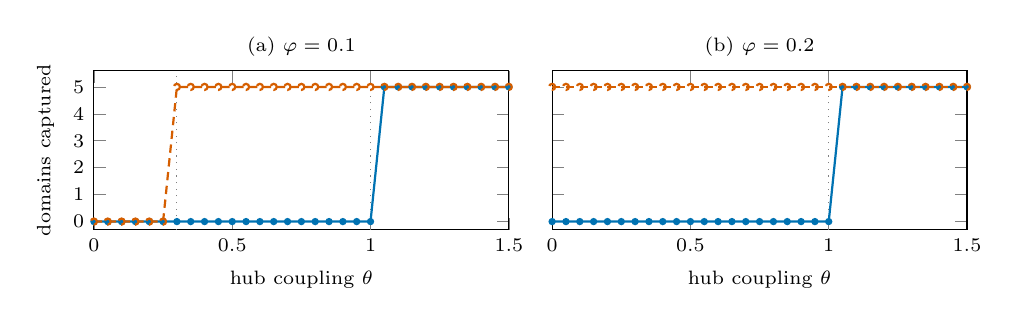
\begin{tikzpicture}
\begin{groupplot}[group style={group size=2 by 1, horizontal sep=0.55cm, y descriptions at=edge left}, width=0.565\columnwidth, height=3.6cm,
  xmin=0, xmax=1.5, ymin=-0.3, ymax=5.6, xtick={0,0.5,1,1.5}, ytick={0,1,2,3,4,5},
  xlabel={hub coupling $\theta$}, tick label style={font=\scriptsize}, label style={font=\scriptsize}, title style={font=\scriptsize, yshift=-1ex}]
\nextgroupplot[title={(a) $\varphi=0.1$}, ylabel={domains captured}]
\addplot[gray, thin, dotted] coordinates {(1,-0.3) (1,5.6)};
\addplot[gray, thin, dotted] coordinates {(0.30,-0.3) (0.30,5.6)};
\addplot[cD, thick, mark=*, mark size=0.9pt] coordinates {(0.0,0) (0.05,0) (0.1,0) (0.15,0) (0.2,0) (0.25,0) (0.3,0) (0.35,0) (0.4,0) (0.45,0) (0.5,0) (0.55,0) (0.6,0) (0.65,0) (0.7,0) (0.75,0) (0.8,0) (0.85,0) (0.9,0) (0.95,0) (1.0,0) (1.05,5) (1.1,5) (1.15,5) (1.2,5) (1.25,5) (1.3,5) (1.35,5) (1.4,5) (1.45,5) (1.5,5)};
\label{pl:up}
\addplot[cH, thick, densely dashed, mark=o, mark size=1.1pt] coordinates {(0.0,0) (0.05,0) (0.1,0) (0.15,0) (0.2,0) (0.25,0) (0.3,5) (0.35,5) (0.4,5) (0.45,5) (0.5,5) (0.55,5) (0.6,5) (0.65,5) (0.7,5) (0.75,5) (0.8,5) (0.85,5) (0.9,5) (0.95,5) (1.0,5) (1.05,5) (1.1,5) (1.15,5) (1.2,5) (1.25,5) (1.3,5) (1.35,5) (1.4,5) (1.45,5) (1.5,5)};
\label{pl:down}
\nextgroupplot[title={(b) $\varphi=0.2$}]
\addplot[gray, thin, dotted] coordinates {(1,-0.3) (1,5.6)};
\addplot[cD, thick, mark=*, mark size=0.9pt] coordinates {(0.0,0) (0.05,0) (0.1,0) (0.15,0) (0.2,0) (0.25,0) (0.3,0) (0.35,0) (0.4,0) (0.45,0) (0.5,0) (0.55,0) (0.6,0) (0.65,0) (0.7,0) (0.75,0) (0.8,0) (0.85,0) (0.9,0) (0.95,0) (1.0,0) (1.05,5) (1.1,5) (1.15,5) (1.2,5) (1.25,5) (1.3,5) (1.35,5) (1.4,5) (1.45,5) (1.5,5)};
\addplot[cH, thick, densely dashed, mark=o, mark size=1.1pt] coordinates {(0.0,5) (0.05,5) (0.1,5) (0.15,5) (0.2,5) (0.25,5) (0.3,5) (0.35,5) (0.4,5) (0.45,5) (0.5,5) (0.55,5) (0.6,5) (0.65,5) (0.7,5) (0.75,5) (0.8,5) (0.85,5) (0.9,5) (0.95,5) (1.0,5) (1.05,5) (1.1,5) (1.15,5) (1.2,5) (1.25,5) (1.3,5) (1.35,5) (1.4,5) (1.45,5) (1.5,5)};
\end{groupplot}
\end{tikzpicture}

\caption{Hysteresis. Domains captured as conversion from development is raised (\ref{pl:up}) and lowered (\ref{pl:down}); dotted lines mark the predicted thresholds $\theta=1$ and $1-R_{ii}-4\varphi$. (a) Capture appears above $\theta=1$ and persists down to $0.26$. (b) The other domains sustain one another and capture survives complete decoupling. Entry rate $\mu=10^{-6}$.}
\label{fig:hyst}
\end{figure}

\section{Experiment Protocol}\label{app:protocol}

\paragraph{Simulated carriers.} Populations of 200 carriers over 4 domains (development tasks; an evaluation rubric; a standard; a curriculum of examples), 60 rounds, 20 seeds per arm. Each carrier has a fixed productivity and a heritable capacity $q\in[0,1]$, mutated with small noise at reproduction. In arm 1, success buys only resources; in arm 2, winners' resources fund changes to next round's rubric, standard and curriculum in proportion to a fixed $q$; in arm 3, $q$ is heritable. Capacity acts only by editing the selection environment, which is logged, never by raising scores directly. Fixed hidden ground truth scores contribution to a shared condition that no in-loop evaluator sees. Manipulations: appropriability of rubric changes (keyed to the editing carrier's style versus applied to all), persistence of edits, an independent evaluator with and without authority to trigger a reset, carrier replacement with rule stocks kept or cleared, and edges cut between domains with explicit re-entry. Pre-registered outcomes: mean capacity, the capacity gradient, persistence of a costly practice after conversion is removed (hysteresis), divergence between in-loop and held-out evaluation, detection time, and recovery after reform.

\paragraph{Language-model agents.} Once the simulated version has fixed the mechanism, replace carriers with agents from at least three model families, with judges drawn from the same and from other families. Estimate $\beta$ as the in-family minus out-of-family score on items with fixed ground truth, and test whether detection delay grows with the in-family share of the panel as Proposition~\ref{prop:detect} predicts. Control for prompt compliance and position effects by randomizing order and paraphrasing instructions.

\section{A Discrete-Time Version}\label{app:discrete}

With rounds $t=0,\dots,T-1$, support $r_{t+1}=(1-\delta)r_t+bq$ from $r_0=0$, and log-fitness increments $f_0-C(q)+\chi ar_t$, the average log-fitness is $f_0-C(q)+\Gamma_Tq$ with $\Gamma_T=(\chi ab/\delta)L_T$ and $L_T=1-[1-(1-\delta)^T]/(\delta T)$. For $a=b=1$ and marginal cost $0.9$: $T=5,\delta=0.2,\chi=0.5$ gives $\Gamma_T=0.82$ (disfavored); $T=20$ gives $1.88$ (favored); faster correction $\delta=0.8$ gives $0.59$; low appropriability $\chi=0.1$ gives $0.38$. If support propagates across domains as $r_{t+1}=Ar_t+qv$ with spectral radius below one and pays $\chi u^\top r$, the long-horizon gradient is $\chi u^\top(I-A)^{-1}v-C'(q)$, whose derivative in $A_{ij}$ is $\chi[u^\top(I-A)^{-1}]_i[(I-A)^{-1}v]_j\ge0$: strengthening any cross-domain path raises the return to capacity, through direct and multi-step paths alike.

\end{document}
